\documentclass[10pt]{article}

% DOCUMENT LAYOUT
%\usepackage{fullpage}
%\usepackage[cm]{fullpage}
%\usepackage[letterpaper, top=0.5in, bottom=0.5in, left=0.5in, right=0.5in]{geometry} 
%\usepackage[letterpaper]{geometry} 
%\geometry{textwidth=5.7in, textheight=9.0in, marginparsep=7pt, marginparwidth=.6in}
%\geometry{textwidth=6.0in, textheight=9.8in, marginparsep=7pt, marginparwidth=.8in}
%\geometry{textwidth=6in, textheight=9.8in, marginparsep=7pt, marginparwidth=.8in}
\setlength\parindent{0in}

%\addtolength{\oddsidemargin}{-.500in}
%\addtolength{\evensidemargin}{-.500in}
%\addtolength{\textwidth}{2.00in}

%\addtolength{\topmargin}{-.875in}
%\addtolength{\textheight}{1.75in}

\addtolength{\topmargin}{-1.125in}
\addtolength{\textheight}{2.0in}

\addtolength{\oddsidemargin}{-.375in}
\addtolength{\evensidemargin}{-.375in}
\addtolength{\textwidth}{1.75in}
\addtolength{\marginparsep}{-10pt}
\addtolength{\marginparwidth}{+15pt}

\usepackage{wrapfig}

\usepackage{chngpage}
\usepackage[export]{adjustbox}

\usepackage{sidecap}
\usepackage[abs]{overpic}
\usepackage{wrapfig}

% SPECIAL FORMATTING
% ---- CUSTOM AMPERSAND
\newcommand{\amper}{{\selectfont\itshape\&}}
% ---- MARGIN YEARS
%\newcommand{\years}[1]{\marginpar{\scriptsize #1}}
\newcommand{\years}[1]{\marginpar{\quad \small #1}}
% ---- TALK COUNTER
\newcounter{talknumber}
\setcounter{talknumber}{1}
% ---- ARTICLE COUNTER
\newcounter{articlenumber}
\setcounter{articlenumber}{1}
%\newcommand{\article}{\noindent\marginpar{\scriptsize \arabic{articlenumber}}\addtocounter{articlenumber}{1}}
\newcommand{\article}[2]{
\noindent\marginpar{
  \parbox[c]{0.25in}{\scriptsize \arabic{articlenumber}} 
  \parbox[c]{0.25in}{\scriptsize \href{#2}{#1}}
}\addtocounter{articlenumber}{1}}
% PAPER DESCRIPTION AND THUMBNAIL IMAGE
\newcommand{\desc}[2]{
\noindent\marginpar{
  \parbox[c]{0.50in}{{\includegraphics[width=0.9in]{thumbnails/{#1}}}}
}{\footnotesize\emph{#2}}}
% NEW ARTICLE STYLE WITH IMAGE AND NO NUMBERS
\newcommand{\newarticle}[5]{
\begin{adjustwidth}{-1in}{-1in}  
\begin{tabular}{p{0.9in}p{7in}}
\parbox[c]{0.9in}{\includegraphics[width=0.9in]{thumbnails/{#1}}} & \parbox[c]{6in}{{#2} $\cdot$ \href{#4}{#3} \\ {\footnotesize\emph {#5}}}
\end{tabular}
\end{adjustwidth}
\vspace{0.2in}
}

% ---- TALKS
\newcommand{\talk}[2]{
\noindent\marginpar{
   \scriptsize \scshape
  #2 \\ #1
}}
\newcommand{\numberedtalk}[2]{
\noindent\marginpar{
  \parbox[c]{0.25in}{\scriptsize \arabic{talknumber}} 
% \parbox[c]{0.5in}{\scriptsize {#2}}
  \parbox[c]{0.5in}{\scriptsize \scshape {#1}}
}\addtocounter{talknumber}{1}}

\newcommand{\newtalk}[3]{
\noindent\marginpar{
   \scriptsize \scshape
  #2 \\ #1
}\spaceTalk\\}

% SPACING
\newcommand{\spaceEd}{\vspace{1ex}}
\newcommand{\spaceRes}{\vspace{1ex}}
\newcommand{\spaceFell}{\vspace{0.5ex}}
\newcommand{\spacePub}{\vspace{0.5ex}}
\newcommand{\spaceTalk}{\vspace{1ex}}
\newcommand{\spaceSoc}{\vspace{0.5ex}}
\newcommand{\spacePost}{\vspace{0.5ex}}

% Modify section spacing
%\usepackage{titlesec}
%\titlespacing*{\section}{0pt}{0.2\baselineskip}{\baselineskip}
%\titlespacing*{\subsection}{0pt}{0.2\baselineskip}{\baselineskip}
%\titlespacing*{\subsubsection}{0pt}{0.2\baselineskip}{\baselineskip}

% GRAPHICS
\usepackage{graphicx}

% HEADINGS
\usepackage{sectsty} 
\usepackage[normalem]{ulem} 

\usepackage{fancyhdr}
\renewcommand{\headrulewidth}{0pt}
\pagestyle{fancy}
\fancyhf{}
%\fancyfoot[LE,CO]{{\small\textsc{John D. Chodera - Sloan Kettering Institute - \thepage}}}%
\rfoot{\small\textsc{John D. Chodera - Sloan Kettering Institute - \thepage}}

% Clean up font spacing with micro type
\usepackage{microtype}

% Use a clean, modern-looking font
\usepackage[default]{lato}
\usepackage[T1]{fontenc}

% Change the appearance of section and subsection headings
\sectionfont{\mdseries\large\underline} 
\subsectionfont{\mdseries\scshape\normalsize} 
\subsubsectionfont{\bfseries\upshape\normalsize} 

% Control tightness of spacing
\renewcommand{\baselinestretch}{1.1}

% PDF SETUP
% ---- FILL IN HERE THE DOC TITLE AND AUTHOR
\usepackage[bookmarks, colorlinks, breaklinks, pdftitle={John D. Chodera - vita},pdfauthor={John D. Chodera}]{hyperref}  
\hypersetup{linkcolor=blue,citecolor=blue,filecolor=black,urlcolor=blue} 

% Change the typewriter font to something nicer.
\usepackage[ttdefault]{sourcecodepro}

% DOCUMENT
\begin{document}
\reversemarginpar
% FILL IN NAME HERE
{\fontseries{eb}\selectfont \LARGE John D. Chodera}\\[1cm]

% FILL IN AUTHOR INFORMATION HERE
\begin{minipage}[t]{2.5in}
%
\includegraphics[width=0.7in,valign=c]{images/john_chodera_sm.pdf}
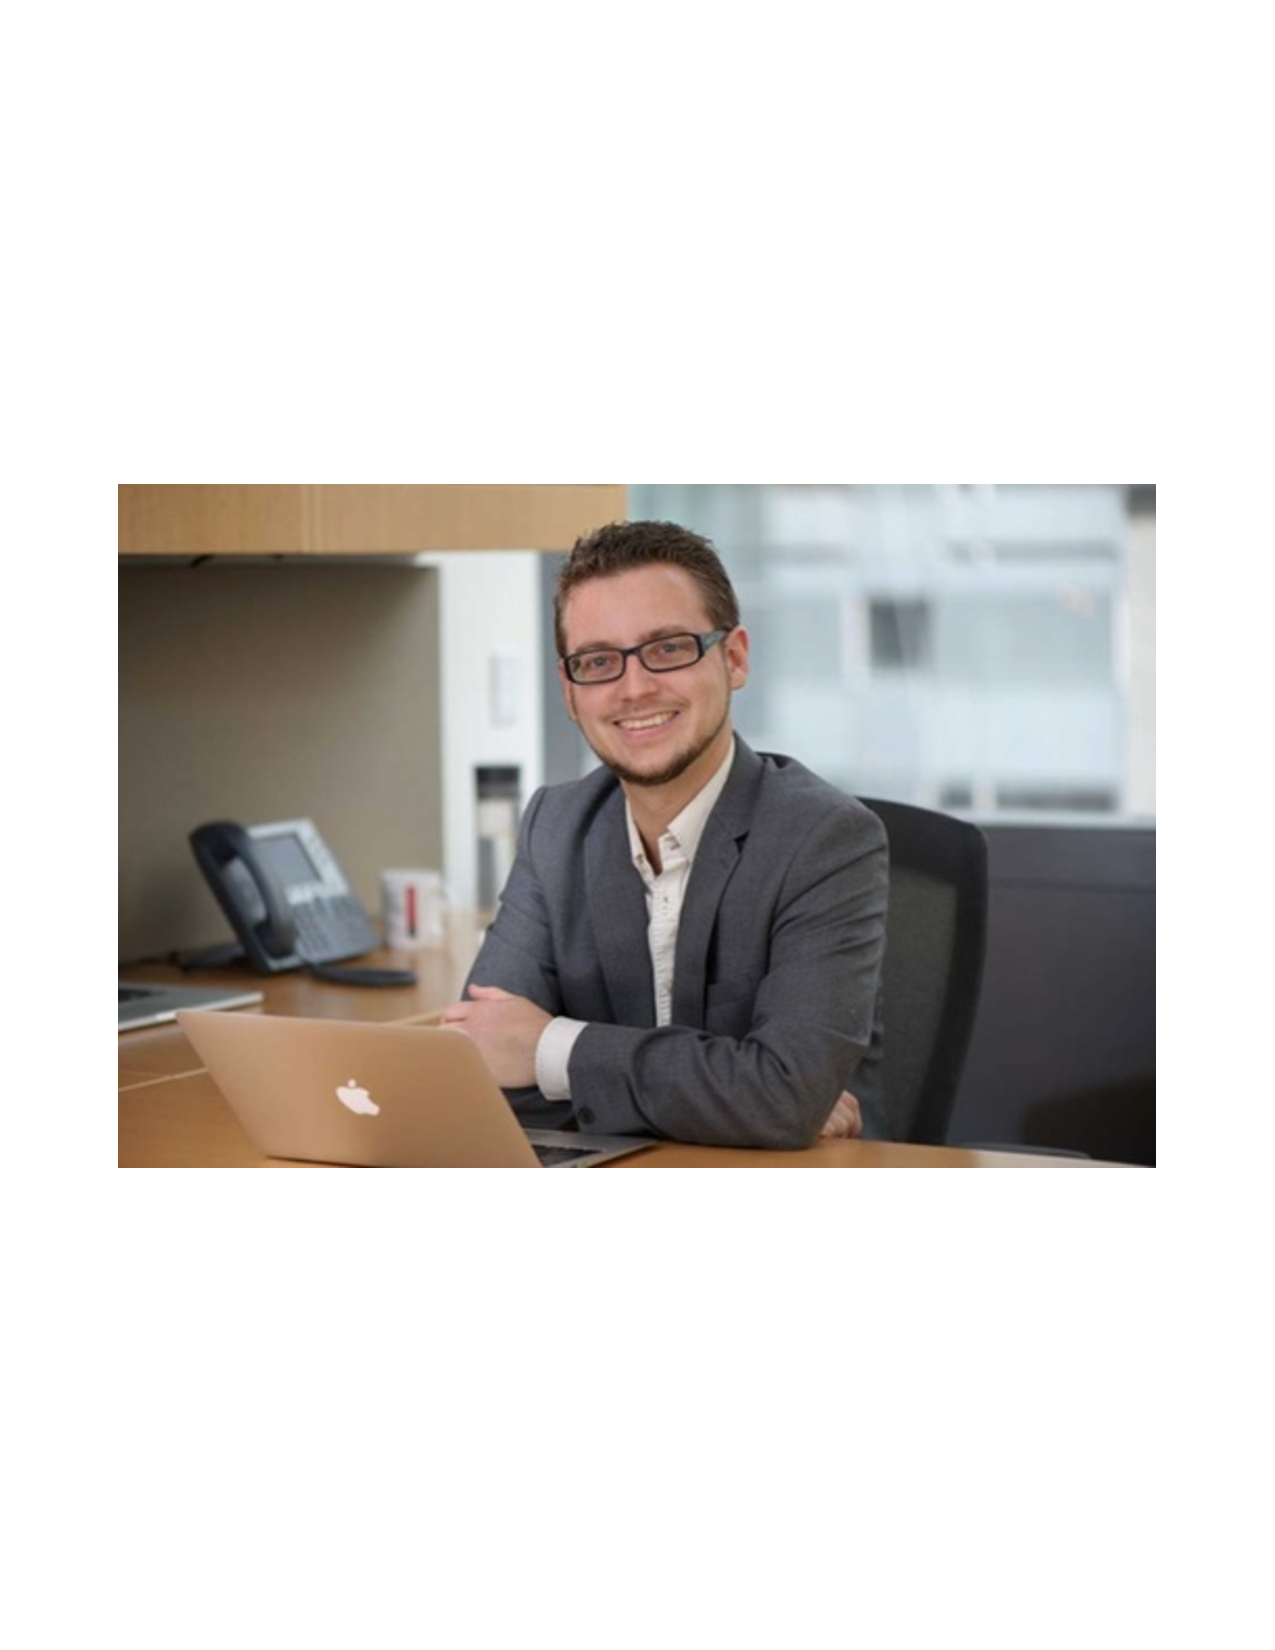
\includegraphics[width=2.5in,valign=c]{images/john_chodera_wide.pdf}
\end{minipage}
\quad
\begin{minipage}[t]{3in}
\begin{tabular}{rl}
{\bf email} & \href{mailto:choderaj@mskcc.org}{\href{mailto:john.chodera@choderalab.org}{john.chodera@choderalab.org}}\\
{\bf url} & \href{http://www.choderalab.org}{\href{http://www.choderalab.org}{http://www.choderalab.org}}\\[0.05in]
{\bf tel} & 646.888.3400\\[0.05in]
{\bf fax} & 510.280.3760 \\[0.05in]
{\bf mobile} & 646.737.3319\\[0.05in]
{\bf post} & 
\parbox[t]{3.0in}{Memorial Sloan Kettering Cancer Center\\
1275 York Ave, Box 357\\
New York, NY 10065}
\end{tabular}
\end{minipage}

% RESEARCH INTERESTS
%\section*{Research interests}
%\noindent {\bf Computational biophysics}, especially \\
%\noindent {\bf Single-molecule biophysics}, including new techniques for interpreting force microscopy \\
%\noindent {\bf Nonequilibrium statistical mechanics}, as tools for single-molecule experimental probes and the design of new algorithms for computational chemistry \\

\section*{Education and positions}

\noindent\years{2013--}{\bf Assistant Professor, Physiology, Biophysics, and Systems Biology Program,\\
Weill Cornell Graduate School of Medical Sciences}\\
\noindent\years{2012--}{\bf Assistant Member, Memorial Sloan-Kettering Cancer Center}\\
\noindent\years{2008--2012}{\bf Independent Distinguished Postdoctoral Fellow, California Institute for Quantitative Biosciences (QB3),\\
University of California, Berkeley}\\
Independent research funding, sponsors \href{http://chem.berkeley.edu/faculty/geissler/index.php}{Phillip L. Geissler} and \href{http://zebra.berkeley.edu/}{Susan Marqusee} \\
%\noindent\years{2011--2012}{\bf \href{http://research.google.com/university/exacycle_program.html}{Google Exacycle Visiting Faculty}} \\
\noindent\years{2006--2008}{\bf Postdoctoral researcher, Department of Chemistry, Stanford University}\\
With \href{http://folding.stanford.edu/Pande/Main}{Vijay S. Pande} (head of \href{http://folding.stanford.edu}{Folding@Home} distributed computing project) \\
\noindent\years{1999--2006}{\bf \textsc{Ph.D.} in Biophysics, University of California, San Francisco}\\
%Dissertation: \href{http://www.dillgroup.ucsf.edu/~jchodera/pubs/pdf/jdcthesis.pdf}{\emph{Master equation models of macromolecular dynamics from atomistic simulation.}} \\
Committee: \href{http://www.dillgroup.org}{Ken A. Dill}, \href{http://jacobsonlab.org/}{Matthew P. Jacobson}, \href{http://folding.stanford.edu/Pande/Main}{Vijay S. Pande}\\
\noindent\years{1995--1999}{\bf \textsc{B.S.} in Biology, California Institute of Technology}\\
Undergraduate research with \href{http://www.its.caltech.edu/~phplab/phplab.html}{Paul H.~Patterson} (\emph{experimental molecular neurobiology}) \\and Jerry E.~Solomon (\emph{computational chemistry}).

\section*{Fellowships and awards}

\noindent\years{2013--2016}Louis V.~Gerstner Young Investigator Award\\
\noindent\years{2013--2014}Google Exacycle for External Faculty\\
\noindent\years{2008--2012}QB3-Berkeley Distinguished Postdoctoral Fellowship, University of California, Berkeley\\
%\noindent\years{2008}Berkeley Mini Stat Mech Meeting Best Poster Prize (second place)\\
\noindent\years{2005--2006}IBM Predoctoral Fellowship\\
\noindent\years{2005}Frank M. Goyan Award for outstanding work in physical chemistry, University of California, San Francisco\\
\noindent\years{2000--2005}Howard Hughes Medical Institute Predoctoral Fellowship\\
\noindent\years{1998--1999}Caltech Upperclass Merit Award Scholarship\\
\noindent\years{1997,$\:$1998}Caltech Summer Undergraduate Research Fellowships

\section*{Research interests}

\noindent{Rational computational design of allosteric small-molecule inhibitors and therapeutics}\\
\noindent{Kinase inhibitor selectivity and evolution of therapeutic resistance in cancer}\\
\noindent{Biomolecular dynamics and conformational heterogeneity}\\
\noindent{Error and uncertainty in biophysical measurements}\\
\noindent{Computational chemistry, molecular modeling, and forcefield development}\\
\noindent{Multiscale modeling of the effects of small molecules on biochemical pathways}\\

\eject

\section*{Publications}

Google Scholar statistics: \href{http://goo.gl/qO0JW}{http://goo.gl/qO0JW}\\
{\small \it h-index: 29 / i10-index: 42}

%{\small \it published peer-reviewed articles: 45 / reviews: 4 / commentaries: 1 / preprints: 6}

{\scriptsize $^*$ asterisk denotes equal contributions}
 
%%%%%%

\subsection*{Published and In Press}

\newarticle{automatic-equilibration-detection.pdf}{{\bf Chodera JD}. A simple method for automated equilibration detection in molecular simulations. \emph{J.~Chem.~Theor.~Comput.}, in press.}{bioRxiv preprint}{http://dx.doi.org/10.1101/021659}{We present a simple approach to automatically determining the equilibrated region of a molecular simulation, a longstanding challenge formerly without a good solution.}

\newarticle{thermoml-benchmark.pdf}{Beauchamp KA, Behr JM, Rustenburg AS, Bayly CI, Kroenlein K, and {\bf Chodera JD}. Towards automated benchmarking of atomistic forcefields: Neat liquid densities and static dielectric constants from the {ThermoML} data archive.  \emph{J. Phys. Chem. B}, 199:12912, 2015.}{DOI}{http://t.co/xhoJzSQKo0}{Molecular mechanics forcefields are critical to computer-guide drug design, but the benchmarking and improvement of these forcefields has been hindered by the lack of high-quality machine-readable physical property datasets. We show how the NIST-curated ThemoML Archive, which stores physical property data in an IUPAC-standard XML format, can eliminate these roadblocks and reveal issues with current generation forcefields.}

\newarticle{L-2HG.pdf}{Intlekofer AM, Dematteo RG, Venetti S, Finley LWS, Lu Chao, Judkins AR, Rutenburg AS, Grinaway PB, {\bf Chodera JD}, Cross JR, and Thompson CB. Hypoxia introduces production of {L-2-Hydroxyglutarate}. {\it Cell Metabolism} 22:1--8, 2015}{DOI}{http://dx.doi.org/10.1016/j.cmet.2015.06.023}{Molecular docking is used to demonstrate the potential for alternative substrate usage by isocitrate dehydrogenases under hypoxic conditions in cancer.}

\newarticle{timestep-rescaling.pdf}{Sivak DA, {\bf Chodera JD}, and Crooks GE. Time step rescaling recovers continuous-time dynamical properties for discrete-time Langevin integration of nonequilibrium systems. {\it J. Phys. Chem. B}, 118:6466--6474, 2014.  William C.~Swope Festschrift}{DOI}{http://dx.doi.org/10.1021/jp411770f}{We derive a simple, easy-to-implement Langevin integrator that has universally useful properties in molecular simulations.}

\newarticle{spectral-rate-theory.pdf}{Prinz J-H, {\bf Chodera JD}, and No\'{e} F. Spectral rate theory for two-state kinetics. {\it Phys.~Rev.~X.} 4:011020, 2014}{DOI}{http://dx.doi.org/10.1103/PhysRevX.4.011020}{We present a new mathematical framework for unifying various two-state rate theories presented in the physical chemistry literature over many decades, and provide a quantitative way to measure reaction coordinate quality.}

\newarticle{identifying-ligand-binding-sites.pdf}{Wang K, {\bf Chodera JD}, Yang Y, and Shirts MR. Identifying ligand binding sites and poses using GPU-accelerated Hamiltonian replica exchange molecular dynamics. {\it J.~Comput.~Aid.~Mol.~Des.}, 27:989--1007, 2013}{DOI}{http://dx.doi.org/10.1007/s10822-013-9689-8}{We show how bound ligand poses can be identified even when the location of the binding sites are unknown using the machinery of alchemical modern free energy calculations on graphics processors.}

\newarticle{iamoeba-water}{Wang L-P, Head-Gordon TL, Ponder JW, Ren P, {\bf Chodera JD}, Eastman PK, Martinez TJ, and Pande VS. Systematic improvement of a classical molecular model of water. {\it J.~Phys.~Chem.~B}, 117:9956--9972, 2013}{DOI}{http://dx.doi.org/10.1021/jp403802c}{A new inexpensive polarizable model of liquid water for next-generation forcefields is derived using an automated parameterization engine.}

\newarticle{nonequilibrium-fluctuation-theorems}{Sivak DA, {\bf Chodera JD}, and Crooks GE. Using nonequilibrium fluctuation theorems to understand and correct errors in equilibrium and nonequilibrium discrete Langevin dynamics simulations. {\it Phys.~Rev.~X.}, 3:011007, 2013}{DOI}{http://dx.doi.org/10.1103/PhysRevX.3.011007}{The finite-timestep errors in molecular dynamics simulations can be interpreted as a form of nonequilibrium work.  We show how this leads to straightforward schemes for correcting for these errors or assessing their impact.}

\newarticle{openmm-logo.pdf}{Eastman P, Friedrichs MS, {\bf Chodera JD}, Radmer RJ, Bruns CM, Ku JP, Beauchamp KA, Lane TJ, Wang L, Shukla D, Tye T, Houston M, Stich T, Klein C, Shirts MR, and Pande VS. OpenMM 4: A reusable, extensible, hardware independent library for high performance molecular simulation. {\it J.~Chem.~Theor.~Comput.}, 9:461, 2012}{DOI}{http://dx.doi.org/10.1021/ct300857j}{We describe the latest version of an open-source, GPU-accelerated library and toolkit for molecular simulation.}

\newarticle{constant-force-feedback.pdf}{Elms PJ, {\bf Chodera JD}, Bustamante CJ, Marqusee S. The limitations of constant-force-feedback experiments. {\it Biophys.~J.}, 103:1490, 2012}{DOI}{http://dx.doi.org/10.1016/j.bpj.2012.06.051}{Popular constant-force-feedback single-molecule experiments can cause severe artifacts in single-molecule force spectroscopy data.  We demonstrate a simple alternative that eliminates these artifacts.}

\newarticle{molten-globule-state.pdf}{Elms PJ, {\bf Chodera JD}, Bustamante C, Marqusee S. The molten globule state is unusually deformable under mechanical force. {\it Proc.~Natl.~Acad.~Sci.~USA.}, 109:3796, 2012}{DOI}{http://dx.doi.org/10.1073/pnas.1115519109}{We measure the physical properties of the molten globule state of apo-myoglobin, and show that it is unusually deformable compared to typical protein native states.}

\newarticle{experimental-observables.pdf}{Pitera JW and {\bf Chodera JD}. On the use of experimental observations to bias simulated ensembles. {\it J.~Chem.~Theor.~Comput.}, 8:3445, 2012}{DOI}{http://dx.doi.org/10.1021/ct300112v}{We show how the concept of maximum entropy can be used to recover unbiased conformational distributions from experimental data, and how this concept relates to the popular `ensemble refinement' schemes for NMR data analysis.}

\newarticle{ribosome-modulates.pdf}{Kaiser CM, Goldman DH, {\bf Chodera JD}, Tinoco I, Jr., and Bustamante C. The ribosome modulates nascent protein folding. {\it Science}, 334:1723, 2011}{DOI}{http://dx.doi.org/10.1126/science.1209740}{Using single-molecule force spectroscopy, we show how the ribosome itself modulates the folding dynamics of nascent protein chains emerging from the exit tunnel.}

\newarticle{splitting-probabilities.pdf}{{\bf Chodera JD} and Pande VS. Splitting probabilities as a test of reaction coordinate choice in single-molecule experiments. {\it Phys.~Rev.~Lett.}, 107:098102, 2011}{DOI}{http://dx.doi.org/10.1103/PhysRevLett.107.098102}{We demonstrate a simple test for identifying poor reaction coordinates in single-molecule experiments.}

\newarticle{itc-enthalpogram.pdf}{Tellinghuisen JT and {\bf Chodera JD}. Systematic errors in isothermal titration calorimetry: Concentrations and baselines. {\it Anal.~Biochem.}, 414:297--299, 2011}{DOI}{http://dx.doi.org/10.1016/j.ab.2011.03.024}{A word of caution about large errors in isothermal titration calorimetry measurements arising from ligand concentration errors.}

\newarticle{multiple-time-slices.pdf}{Minh DDL, {\bf Chodera JD}. Estimating equilibrium ensemble averages using multiple time slices from driven nonequilibrium processes: Theory and application to free energies, moments, and thermodynamic length in single-molecule pulling experiments. {\it J.~Chem.~Phys.} 134:024111, 2011}{DOI}{http://dx.doi.org/10.1063/1.3516517}{We derive a new estimator for estimating equilibrium expectations from nonequilibrium experiments, and show how it can be used to estimate a variety of useful quantities in simulated single-molecule force spectroscopy experiments.}

\newarticle{ncmc.pdf}{Nilmeier JP, Crooks GE, Minh DDL, and {\bf Chodera JD}. Nonequilibrium candidate Monte Carlo is an efficient tool for equilibrium simulation. {\it Proc.~Natl.~Acad.~Sci.~USA.}, 108:E1009, 2011}{DOI}{http://dx.doi.org/10.1073/pnas.1106094108}{We present a significant generalization of Monte Carlo methods that provide an enormously useful tool for enhancing the efficiency of molecular simulations and enabling molecular design.}

\newarticle{parallel-tempering.pdf}{Prinz J-H, {\bf Chodera JD}, Pande VS, Smith JC, and No\'{e} F. Optimal use of data in parallel tempering simulations for the construction of discrete-state Markov models of biomolecular dynamics. \emph{J.~Chem.~Phys.} 134:244108, 2011}{DOI}{http://dx.doi.org/10.1063/1.3592153}{We demonstrate how multitemperature data from parallel tempering simulations can be used to construct fully temperature-dependent models of the dynamics of biomolecular systems.}

\newarticle{dynamical-reweighting.pdf}{{\bf Chodera JD}, Swope WC, No\'{e} F, Prinz J-H, Shirts MR, and Pande VS. Dynamical reweighting: Improved estimates for dynamical properties from simulations at multiple temperatures. \emph{J. Chem. Phys.} 134:244107, 2011}{DOI}{http://dx.doi.org/10.1063/1.3592152}{We describe how reweighing techniques can provide optimal estimates of temperature-dependent dynamical properties from simulations conducted at multiple temperatures.}

\newarticle{dynamical-fingerprints.pdf}{No\'{e} F, Doose S, Daidone I, L\"{o}llmann M, Sauer M, {\bf Chodera JD}, and Smith JC. Dynamical fingerprints: A theoretical framework for understanding biomolecular processes by combination of simulation and kinetic experiments. \emph{Proc.~Natl.~Acad.~Sci.~USA}, 108:4822, 2011}{DOI}{http://dx.doi.org/10.1073/pnas.1004646108}{We present a new framework for comparing essential features of the dynamics between experiment and simulation to identify the kinetics processes contributing to individual relaxation timescales in perturbation-response or correlation spectroscopy experiments.}

\newarticle{gibbs-sampling.pdf}{{\bf Chodera JD} and Shirts MR. Replica exchange and expanded ensemble simulations as Gibbs sampling: Simple improvements for enhanced mixing. \emph{J.~Chem.~Phys.}, 135:194110, 2011}{DOI}{http://dx.doi.org/10.1063/1.3660669}{We show how a simple change to the way exchanges are handled in the popular replica-exchange simulation methodology can enormously increase efficiency at no increase in computational cost.}

\newarticle{current-status-amoeba.pdf}{Ponder JW, Wu C, Ren P, Pande VS, {\bf Chodera JD}, Mobley DL, Schnieders MJ, Haque I, Lambrecht DS, DiStasio RA Jr., Head-Gordon M,  Clark GNI, Johnson ME, and Head-Gordon T. Current status of the AMOEBA polarizable force field. {\it J.~Phys.~Chem.~B} 114:2549, 2010}{DOI}{http://dx.doi.org/10.1021/jp910674d}{A report on the status of the AMOEBA polarizable force field and its ability to reproduce a diverse set of physical chemical phenomenon to high accuracy.}

\newarticle{observable-uncertainty.pdf}{{\bf Chodera JD} and No\'e F. Probability distributions of molecular observables computed from Markov models.~II.~Uncertainties in observables and their time-evolution. \emph{J. Chem. Phys.} 133:105102, 2010}{DOI}{http://dx.doi.org/10.1063/1.3463406}{A simple Bayesian approach for the modeling of statistical uncertainties in kinetic and equilibrium quantities computed from Markov state models of biomolecular dynamics.}

\newarticle{pcna-cover.pdf}{Adelman JL, {\bf Chodera JD}, Kuo IW, Miller TF, and Barsky D. The mechanical properties of PCNA: Implications for the loading and function of a DNA sliding clamp. {\it Biophys. J.} 98:3062, 2010}{DOI}{http://dx.doi.org/10.1016/j.bpj.2010.03.056}{Molecular simulations of the PCNA clamp responsible for DNA polymerase processivity show a surprisingly small energetic penalty for the deformation required for clamp loading.  Featured on issue cover.}

\newarticle{bayesian-comparison-markov-models.pdf}{Bacallado S, {\bf Chodera JD}, and Pande VS. Bayesian comparison of Markov models of molecular dynamics with detailed balance constraint. \emph{J.~Chem.~Phys.} 131:045106, 2009}{DOI}{http://dx.doi.org/10.1063/1.3192309}{A Bayesian scheme for comparing state space decompositions for Markov state models of biomolecular dynamics that incorporates the fact that physical systems must obey detailed balance.  This paper utilizes recent results from Markov chain theory on edge-reinforced random walks.}

\newarticle{optimal-estimates-nonequilibrium.pdf}{Minh DDL, {\bf Chodera JD}. Optimal estimators and asymptotic variances for nonequilibrium path-ensemble averages. {\it J.~Chem.~Phys.} 131:134110, 2009}{DOI}{http://dx.doi.org/10.1063/1.3242285}{We derive an optimal estimator and corresponding statistical uncertainties for inferring expectations of bidirectional nonequilibrium processes.  These estimators have widespread applicability in single-molecule biophysical force-spectroscopy experiments and nonequilibrium molecular simulations.}

\newarticle{mbar-equation.pdf}{Shirts MR, {\bf Chodera JD}. Statistically optimal analysis of samples from multiple equilibrium states. {\it J.~Chem.~Phys.} 129:124105, 2008}{DOI}{http://dx.doi.org/10.1063/1.2978177}{We present a highly general, statistically optimal approach for producing estimates of free energies and equilibrium expectations from multiple simulations that provably extracts all useful information from the data.}

\newarticle{small-molecule-solvation.pdf}{Nicholls A*, Mobley DL*, Guthrie JP, {\bf Chodera JD}, and Pande VS. Predicting small-molecule solvation free energies: A blind challenge test for computational chemistry. {\it J.~Med.~Chem.} 51:769--779, 2008}{DOI}{http://dx.doi.org/10.1021/jm070549+}{A blind evaluation of the accuracy of alchemical free energy methods for computing gas-to-water transfer free energies (solvation free energies) of small molecules demonstrates that modern forcefields are likely sufficiently accurate to be useful in drug design.}

\newarticle{entropy-solvation.pdf}{Mobley DL, Dill KA, and {\bf Chodera JD}. Treating entropy and conformational changes in implicit solvent simulations of small molecules. {\it J.~Phys.~Chem.~B} 112(3):938--946, 2008}{DOI}{http://dx.doi.org/10.1021/jp0764384}{An quantitative examination of how much conformational entropy contributes to hydration free energies of small molecules, with implications for ligand binding.}

\newarticle{long-range-dispersion-correction.pdf}{Shirts MR*, Mobley DL*, {\bf Chodera JD}, and Pande VS. Accurate and efficient corrections for missing dispersion interactions in molecular simulations.  {\it J.~Phys.~Chem.~B} 111(45):13052--13063, 2007}{DOI}{http://dx.doi.org/10.1021/jp0735987}{We identify a major source of systematic error in absolute alchemical free energy calculations of ligand binding and show how a simple procedure can inexpensively and accurately eliminate it.}

\newarticle{charge-models.pdf}{Mobley DL, Dumont E, {\bf Chodera JD}, Bayly CI, Cooper MD, and Dill KA. Comparison of charge models for fixed-charge force fields: Small-molecule hydration free energies in explicit solvent.  \emph{J.~Phys.~Chem.~B} 111:2242--2254, 2007}{DOI}{http://dx.doi.org/10.1021/jp0667442}{We compare a number of popular methods for deriving charge models for small molecules, deriving lessons about best practices for accurate simulations.}

\newarticle{t4-lysozyme-l99a.pdf}{Mobley DL, Graves AP, {\bf Chodera JD}, McReynolds AC, Shoichet BK, and Dill KA. Predicting absolute ligand binding free energies to a simple model site. {\it J.~Mol.~Biol.} 371(4):1118--1134, 2007}{DOI}{http://dx.doi.org/10.1016/j.jmb.2007.06.002}{We show how alchemical free energy calculations are capable of accurate blind prediction of small-molecule binding affinities to a simple model protein binding site.}

\newarticle{t4-lysozyme-val111}{Mobley DL, {\bf Chodera JD}, and Dill KA. Confine-and-release method: Obtaining correct binding free energies in the presence of protein conformational change. {\it J.~Chem.~Theor.~Comput.} 3(4):1231--1235, 2007}{DOI}{http://dx.doi.org/10.1021/ct700032n}{We present a general scheme for obtaining correct ligand binding affinities when protein conformational change is implicated in ligand binding.}

\newarticle{automatic-state-decomposition-trpzip2.pdf}{{\bf Chodera JD}*, Singhal N*, Swope WC, Pitera JW, Pande VS, and Dill KA. Automatic discovery of metastable states for the construction of Markov models of macromolecular conformational dynamics. {\it J.~Chem.~Phys.} 126:155101, 2007}{DOI}{http://dx.doi.org/10.1063/1.2714538}{Proposing one of the first automated algorithms for discovering kinetically metastable states of biomolecules from molecular simulations, this paper shows how many biomolecules can possess numerous distinct long-lived conformational states even though the the equilibrium populations of these states may too small for standard structural biology techniques to detect.}

\newarticle{zipping-assembly.pdf}{Ozkan SB, Wu GA, {\bf Chodera JD}, and Dill KA. Protein Folding by Zipping and Assembly. \emph{Proc.~Natl.~Acad.~Sci.~USA} 104(29):11987--11992, 2007}{DOI}{http://dx.doi.org/10.1073/pnas.0703700104}{A review of the utility of the proposed zipping and assembly mechanism for the concomitant formation of secondary and tertiary structure in protein folding for predicting folding pathways and native structures.}

\newarticle{alanine-dipeptide-2dpmf.pdf}{{\bf Chodera JD}, W. C. Swope, J. W. Pitera, C. Seok, and K. A. Dill. Use of the weighted histogram analysis method for the analysis of simulated and parallel tempering simulations. \emph{J.~Chem.~Theor.~Comput.} 3(1):26--41, 2007}{DOI}{http://dx.doi.org/10.1021/ct0502864}{The weighted histogram analysis method (WHAM), a mainstay of molecular dynamics simulation analysis, is thoroughly explained and modernized for the analysis of simulated and parallel tempering simulation data.}

\newarticle{orientational-restraints.pdf}{Mobley DL, {\bf Chodera JD}, and Dill KA. On the use of orientational restraints and symmetry corrections in alchemical free energy calculations. {\it J.~Chem.~Phys.} 125:084902, 2006}{DOI}{http://dx.doi.org/10.1063/1.2221683}{We illustrate how orientational restraints can be used to greatly reduce the computational effort in alchemical calculations of ligand binding free energies, and clarify how symmetry corrections are necessary when molecules contain symmetric or pseudosymmetric substituents.}

\newarticle{alanine-dipeptide.pdf}{{\bf Chodera JD}, Swope WC, Pitera JW, and Dill KA. Long-time protein folding dynamics from short-time molecular dynamics simulations. {\it Multiscale~Model.~Simul.} 5(4):1214--1226, 2006}{DOI}{http://dx.doi.org/10.1137/06065146X}{We show how the long-time dynamics of biomolecular systems can be recapitulated from statistics collected from short molecular simulations sampling transitions between kinetically metastable states.}

\newarticle{moped.pdf}{Seok C, Rosen JB, {\bf Chodera JD}, Dill KA. MOPED: Method for optimizing physical energy parameters using decoys. {\it J.~Comput.~Chem.} 24(1):89--97, 2003}{DOI}{http://dx.doi.org/10.1002/jcc.10124}{We propose a novel way to optimize parameters for a physical energy function for protein folding studies by making use of `decoy' structures.}

\newarticle{odcase.pdf}{Lee TS$^*$, Chong LT$^*$, {\bf Chodera JD}, and Kollman PA. An alternative explanation for the catalytic proficiency of orotidine 5'-phosphate decarboxylase. {\it J.~Am.~Chem.~Soc.} 123(51):12837-12848, 2001}{DOI}{http://dx.doi.org/10.1021/ja011096f}{A combined QM and MD analysis of potential plausible mechanisms to explain the enormous catalytic acceleration of one of the most proficient enzymes known.}

\eject

%%%%%%%%%%%%

\section*{Submitted and Under Review}

\newarticle{ensembler.pdf}{Parton DL, Grinaway PB, Hanson SM, Beauchamp KA, and {\bf Chodera JD}. Ensembler: Enabling high-throughput molecular simulations at the superfamily scale}{bioR$\chi$v}{http://dx.doi.org/10.1101/018036} {We demonstrate a new tool that enables---for the first time---massively parallel molecular simulation studies of biomolecular dynamics at the superfamily scale, illustrating its application to protein tyrosine kinases, an important class of drug targets in cancer.}

\newarticle{itc-worksheet}{Boyce SE, Tellinghuisen JT, and {\bf Chodera JD}. Avoiding accuracy-limiting pitfalls in the study of protein-ligand interactions with isothermal titration calorimetry}{bioR$\chi$v}{http://dx.doi.org/10.1101/018036}{We demonstrate how to avoid accuracy-limiting problems in standard isothermal calorimetry experiments as well as capture the primary sources of uncertainty in thermodynamic parameters.}

\newarticle{bhmm.pdf}{{\bf Chodera JD}, No\'{e} F, Hinrichs NS, Keller B, Elms PJ, Kaiser CM, Ewall-Wice A, Marqusee S, and Bustamante C. Bayesian hidden Markov model analysis of single-molecule biophysical experiments}{ar$\chi$iv}{http://arxiv.org/find/all/1/all:+chodera/0/1/0/all/0/1}{We present a Bayesian hidden Markov model analysis scheme that allows biomolecular conformational dynamics to be inferred from single-molecule trajectories.}

\newarticle{robust-rate-estimates.pdf}{{\bf Chodera JD}, Elms PJ, Swope WC, Prinz J-H, Marqusee S, Bustamante C, No\'{e} F, and Pande VS. A robust approach to estimating rates from time-correlation functions}{ar$\chi$iv}{http://arxiv.org/abs/1108.2304}{We present a simple, robust approach to estimating two-state rate constants from experimental or simulation data.}

\eject

%%%%%%%%%%%%

\section*{Reviews and Commentaries}

\newarticle{msm-projection.pdf}{{\bf Chodera JD} and No\'{e} F. Markov state models of biomolecular conformational dynamics. \emph{Curr.~Opin.~Struct.~Biol.}, 25:135--144, 2014.}{DOI}{http://dx.doi.org/10.1016/j.sbi.2014.04.002}{A review of the exciting developments in the stochastic modeling of biomolecular dynamics over the last few years.}

\newarticle{entropy-enthalpy-compensation.pdf}{{\bf Chodera JD} and Mobley DL. Entropy-enthalpy compensation: Role and ramifications for rational ligand design. {\it Annu.~Rev.~Biophys.}, 42:121, 2013}{DOI}{http://dx.doi.org/10.1146/annurev-biophys-083012-130318}{Entropy-enthalpy compensation is likely a universal phenomena, but not as severe as widely thought, and likely not of enormous concern for drug discovery and ligand design.}

\newarticle{alchemical-methods.pdf}{{\bf Chodera JD}, Mobley DL, Shirts MR, Dixon RW, Branson KM, and Pande VS. Free energy methods in drug discovery and design: Progress and challenges. {\it Curr.~Opin.~Struct.~Biol.}, 21:150--160, 2011}{DOI}{http://dx.doi.org/10.1016/j.sbi.2011.01.011}{A review of the opportunities and challenges for alchemical free energy calculations in drug discovery and design.}

\newarticle{markov-model-generation-3.pdf}{Prinz JH, Wu H, Sarich M, Keller B, Fischbach M, Held M, {\bf Chodera JD}, Sch\"{u}tte, and No\'{e} F. Markov models of molecular kinetics: Generation and validation. \emph{J.~Chem.~Phys.} 134:174105, 2011}{DOI}{http://dx.doi.org/10.1063/1.3565032}{A review of current best practices for the generation and validation of Markov state models for describing the stochastic dynamics of biomolecular systems.}

\newarticle{social-network.pdf}{{\bf Chodera JD} and Pande VS. The Social Network (of protein conformations). \emph{Proc.~Natl.~Acad. Sci.~USA} 108:12969, 2011}{DOI}{http://dx.doi.org/10.1073/pnas.1109571108}{A new methodology for mapping protein conformational spaces is reminiscent of how we use two-dimensional maps to navigate a three-dimensional world.}

\newarticle{binding-free-energy.pdf}{Shirts MR, Mobley DL, {\bf Chodera JD}. Alchemical free energy calculations: Ready for prime time? {\it Ann.~Rep.~Comput.~Chem.} 3:41--59, 2007}{DOI}{http://dx.doi.org/10.1016/S1574-1400(07)03004-6}{A review of current alchemical free energy methodologies assessing whether they are ready for practical use in drug discovery and ligand design.}

\newarticle{folding-funnel.pdf}{Dill KA, Ozkan SB, Weikl TR, {\bf Chodera JD}, and Voelz VA. The protein folding problem: When will it be solved? \emph{Curr.~Opin.~Struct.~Biol.} 17(3):342--346, 2007}{DOI}{http://dx.doi.org/10.1016/j.sbi.2007.06.001}{A review of the current state of the protein folding problem.}

\eject
%%%%%%%%%%%%

\section*{Conferences organized}

\talk{May 2016}{Boston}Free Energy Methods in Drug Design Workshop \\ {\small Hosted at Vertex Pharmaceuticals}\vspace{0.5ex}

\talk{May 2016}{Cambridge, MA}Markov State Models in Drug Design Workshop \\ {\small Hosted at Novartis}\vspace{0.5ex}

\talk{Sep 2015}{Berlin}World Molecular Kinetics Workshop 2015 \\ {\small Hosted at Freie Universit\"{a}t Berlin} \vspace{0.5ex}

\talk{May 2014}{Boston}Free Energy Methods in Drug Design Workshop \\ {\small Hosted at Vertex Pharmaceuticals}\vspace{0.5ex}

\talk{Sep 2013}{Berlin}World Molecular Kinetics Workshop 2013 \\ {\small Hosted at Freie Universit\"{a}t Berlin} \vspace{0.5ex}

\talk{May 2012}{Cambridge, MA}Free Energy Methods in Drug Design Workshop \\ {\small Hosted at Vertex Pharmaceuticals}\vspace{0.5ex}

\talk{Sep 2011}{Berlin}World Molecular Kinetics Workshop 2011 \\ {\small Hosted at Freie Universit\"{a}t Berlin} \vspace{0.5ex}

\talk{May 2010}{Cambridge, MA}Free Energy Methods in Drug Design Workshop \\ {\small Hosted at Vertex Pharmaceuticals}\vspace{0.5ex}

\talk{May 2009}{Berlin}World Molecular Kinetics Workshop 2009 \\ {\small Hosted at Freie Universit\"{a}t Berlin}

%% TALKS

%\section*{Invited presentations}
%
%\numberedtalk{Jul 2013}{Mount Snow, VT}Computer Aided Drug Discovery GRC\\ {\small Experimental (T)error: Strategies for coping with data in an uncertain world} \vspace{0.5ex}
%
%\numberedtalk{Jul 2013}{Snowmass, CO}Free energy workshop.\\ {\small Redesigning drug design} \vspace{0.5ex}
%
%\numberedtalk{Apr 2013}{Merced}Chemistry Departmental Seminar, UC Merced.\\ {\small Redesigning drug design} \vspace{0.5ex}
%
%\numberedtalk{Jan 2013}{College Park}Statistical Mechanics Seminar Series, University of Maryland.\\ {\small New applications of nonequilibrium fluctuation theorems in single-molecule biophysics and molecular simulation} \vspace{0.5ex}
%
%\numberedtalk{Sep 2012}{Marconi Center}UC Berkeley Biophysics Retreat.\\ {\small Redesigning drug design} \vspace{0.5ex}
%
%\numberedtalk{Sep 2012}{Skytop}MSKCC cBio Retreat.\\ {\small Redesigning drug design} \vspace{0.5ex}
%
%\numberedtalk{Sep 2012}{Zurich}CECAM Protein Folding Workshop, ETH Zurich.\\ {\small New techniques for extracting insight from single-molecule force spectroscopy} \vspace{0.5ex}
%
%\numberedtalk{Feb 2012}{Schr\"dingier}Schr\"{o}dinger, New York\\ {\small Redesigning drug design} \vspace{0.5ex}
%
%\numberedtalk{Feb 2012}{Berlin}Freie Universit\"{a}t Berlin, MATHEON\\ {\small How do biomolecules move?} \vspace{0.5ex}
%
%\numberedtalk{Jan 2012}{Berkeley}Physics Departmental Seminar, UC Berkeley \\ {\small How do biomolecules move?} \vspace{0.5ex}
%
%\numberedtalk{Jan 2012}{Berkeley}Berkeley Mini Stat Mech Meeting\\ {\small Unraveling the statistical mechanics of biomolecules with force spectroscopy} \vspace{0.5ex}
%
%\numberedtalk{Sep 2011}{Berlin}World Molecular Kinetics Workshop, Berlin\\ {\small New techniques for nonequilibrium force spectroscopy} \vspace{0.5ex}
%
%\numberedtalk{Aug 2011}{Johns Hopkins}Johns Hopkins University\\ {\small Toward multiscale modeling of the effects of small molecules on cellular pathways}\vspace{0.5ex}
%
%\numberedtalk{Mar 2011}{UCSF}University of California, San Francisco\\ {\small Pushing the boundaries of single-molecule force spectroscopy} \vspace{0.5ex}
%
%\numberedtalk{Jan 2011}{MIT}Physical Chemistry Seminar, MIT \\ {\small How do biomolecules move?} \vspace{0.5ex}
%
%\numberedtalk{Jul 2010}{New York}Schr\"{o}dinger, New York \\ {\small Alchemical free energy methods for drug discovery} \vspace{0.5ex}
%
%\numberedtalk{Jun 2010}{Edinburgh}Multiscale Molecular Modeling (M3) meeting, Edinburgh \\ {\small Optimal estimates of dynamical properties} \vspace{0.5ex}
%
%\eject
%
%\numberedtalk{Jan 2010}{Berkeley}Berkeley Mini Stat Mech Meeting, TPS Satellite Meeting, Berkeley \\ {\small Optimal estimation from multiple path sampling simulations} \vspace{0.5ex}
%
%\numberedtalk{Dec 2009}{Cambridge}Vertex Pharmaceuticals, Cambridge MA \\ {\small Entropy-enthalpy compensation: Not even wrong?} \vspace{0.5ex}
%
%\numberedtalk{Apr 2009}{Purdue}Purdue University\\ {\small How do biomolecules move?} \vspace{0.5ex}
%
%\numberedtalk{Apr 2009}{Notre Dame}University of Notre Dame\\ {\small How do biomolecules move?} \vspace{0.5ex}
%
%\numberedtalk{Apr 2009}{Berlin}Freie Universit\"{a}t Berlin, MATHEON\\ {\small Estimators for equilibrium and nonequilibrium experiments} \vspace{0.5ex}
%
%\numberedtalk{Mar 2009}{Miami}SIAM National Meeting, Miami\\ {\small } {\small Bridging between atomistic simulation and physical experiments with master equation models} \vspace{0.5ex}
%
%\numberedtalk{Feb 2009}{UCLA}IPAM Rare Events in High-Dimensional Systems, UCLA\\ {\small Bridging between atomistic simulation and physical experiments with master equation models}\vspace{0.5ex}
%
%\numberedtalk{Jul 2008}{Telluride}Telluride meeting on Enhanced Sampling Methods\\ {\small Statistically optimal estimates from multiple equilibrium samples} \vspace{0.5ex}
%
%\numberedtalk{Jun 2008}{Banff}BIRS Workshop on Mathematical Methods for Free Energy Calculations in Molecular Systems\\ {\small Statistically optimal estimates from equilibrium and nonequilibrium measurements} \vspace{0.5ex}
%
%\numberedtalk{Apr 2008}{Stanford}Gromacs Workshop, Stanford\\ {\small Alchemical free energy calculations with {\tt gromacs}}\vspace{0.5ex}
%
%\numberedtalk{Feb 2008}{Vienna}ESI Workshop on Metastability and Rare Events in Complex Systems, Vienna\\ {\small Master equation models of protein folding and dynamics from atomistic molecular dynamics simulation} \vspace{0.5ex}
%
%\numberedtalk{Aug 2007}{Boston}ACS National Meeting, Boston\\ {\small Bridging timescales between atomistic simulation and experiments} \vspace{0.5ex}
%
%%\numberedtalk{Mar 2007}{Chicago}ACS National Meeting\\ {\small Accuracy and reliability in molecular simulation. \emph{(Substituting for Vijay S. Pande)}} \vspace{0.5ex}
%
%\numberedtalk{Sep 2006}{Heidelberg}MMS06 Workshop, Heidelberg\\ {\small Describing peptide and protein folding dynamics by discrete-state master equation models} \vspace{0.5ex}
%
%\numberedtalk{Dec 2003}{San Diego}Burroughs Wellcome Fund, Interfaces in Science Program retreat, San Diego\\ {\small Constructing master equation models of protein dynamics from atomistic simulation} \vspace{0.5ex}
%
%\numberedtalk{Mar 2003}{New York}ACS National Meeting, New York\\ {\small Extracting dynamical information from parallel tempering simulations}
%
%%%%%%%%%%%

%\talk{Sep 2011}{Berlin}World Molecular Kinetics Workshop\\ {\small New techniques for nonequilibrium force spectroscopy} \vspace{0.5ex}
%
%\talk{Aug 2011}{Johns Hopkins}Invited talk, Johns Hopkins University\\ {\small Toward multiscale modeling of the effects of small molecules on cellular pathways}\vspace{0.5ex}
%
%\talk{Mar 2011}{UCSF}Invited talk, UCSF\\ {\small Pushing the boundaries of single-molecule force spectroscopy} \vspace{0.5ex}
%
%\eject
%
%\talk{Jan 2011}{MIT}Physical Chemistry Seminar, MIT \\ {\small How do biomolecules move?} \vspace{0.5ex}
%
%\talk{Jul 2010}{New York}Invited talk, Schr\"{o}dinger \\ {\small Alchemical free energy methods for drug discovery} \vspace{0.5ex}
%
%\talk{Jun 2010}{Edinburgh}Multiscale Molecular Modeling (M3) meeting \\ {\small Optimal estimates of dynamical properties} \vspace{0.5ex}
%
%\talk{Jan 2010}{Berkeley}Berkeley Mini Stat Mech Meeting, TPS Satellite Meeting \\ {\small Optimal estimation from multiple path sampling simulations} \vspace{0.5ex}
%
%\talk{Dec 2009}{Boston}Vertex Pharmaceuticals \\ {\small Entropy-enthalpy compensation: Not even wrong?} \vspace{0.5ex}
%
%\talk{Apr 2009}{Purdue}Invited talk, Purdue University\\ {\small How do biomolecules move?} \vspace{0.5ex}
%
%\talk{Apr 2009}{Notre Dame}Invited talk, University of Notre Dame\\ {\small How do biomolecules move?} \vspace{0.5ex}
%
%\talk{Apr 2009}{Berlin}Freie Universit\"{a}t Berlin, MATHEON\\ {\small Estimators for equilibrium and nonequilibrium experiments} \vspace{0.5ex}
%
%\talk{Mar 2009}{Miami}SIAM National Meeting - State Space Decomposition Methods in Molecular Simulations\\ {\small } {\small Bridging between atomistic simulation and physical experiments with master equation models} \vspace{0.5ex}
%
%\talk{Feb 2009}{UCLA}IPAM Rare Events in High-Dimensional Systems\\ {\small Bridging between atomistic simulation and physical experiments with master equation models}\vspace{0.5ex}
%
%\talk{Jul 2008}{Telluride}Telluride meeting on Enhanced Sampling Methods \\ {\small Statistically optimal estimates from multiple equilibrium samples.} \vspace{0.5ex}
%
%\talk{Jun 2008}{Banff}BIRS Workshop on Mathematical Methods for Free Energy Calculations in Molecular Systems\\ {\small Statistically optimal estimates from equilibrium and nonequilibrium measurements.} \vspace{0.5ex}
%
%\talk{Apr 2008}{Stanford}Gromacs Workshop\\ {\small Alchemical free energy calculations with {\tt gromacs}}\vspace{0.5ex}
%
%\talk{Feb 2008}{Vienna}ESI Workshop on Metastability and Rare Events in Complex Systems\\ {\small Master equation models of protein folding and dynamics from atomistic molecular dynamics simulation} \vspace{0.5ex}
%
%\talk{Aug 2007}{Boston}ACS National Meeting\\ {\small Bridging timescales between atomistic simulation and experiments.} \vspace{0.5ex}
%
%%\talk{Mar 2007}{Chicago}ACS National Meeting\\ {\small Accuracy and reliability in molecular simulation. \emph{(Substituting for Vijay S. Pande)}} \vspace{0.5ex}
%
%\talk{Sep 2006}{Heidelberg}MMS06 Workshop\\ {\small Describing peptide and protein folding dynamics by discrete-state master equation models} \vspace{0.5ex}
%
%\talk{Dec 2003}{San Diego}Burroughs Wellcome Fund, Interfaces in Science Program retreat.\\ {\small Constructing master equation models of protein dynamics from atomistic simulation.} \vspace{0.5ex}
%
%\talk{Mar 2003}{New York}ACS National Meeting\\ {\small Extracting dynamical information from parallel tempering simulations.}
%

%\section*{Teaching experience}
%
%\noindent\years{\scshape 2013-}Faculty, Tri-Institutional Training Program in Computational Biology and Medicine (CBM)\\
%\noindent\years{\scshape 2013-}Faculty, Tri-Institutional Training Program in Chemical Biology (TPCB)\\
%\noindent\years{\scshape Fall 2006}MathBio Boot Camp, UCSF Biophysics. \\
%\noindent\years{\scshape Fall 2003}Teaching Assistant, UCSF BP 206, Computation of Biological Molecules, Matthew P. Jacobson. \\
%\noindent\years{\scshape Fall 2000}Teaching Assistant, UCSF Chem 241, Molecular Thermodynamics / Stat Mech, Ken A. Dill.

%\section*{Research and Computing Grants}
%
%\noindent {\bf Astra-Zeneca iMED Collaboration Award} (2015--2016) \\
%{\small Understanding slow off-rate inhibition in CK2 and SYK} 
%
%\noindent {\bf Functional Genomics Initiative (FGI) Award} (2015--2017) \\
%{\small Characterization of cancer-derived mTOR mutants for precision therapeutics} 
%
%\noindent {\bf Functional Genomics Initiative (FGI) Rapid Response Award} (2015--2016) \\
%{\small Assessing the biophysical impact of clinical kinase mutations on drug binding affinity} 
%
%\noindent {\bf Starr Cancer Foundation} (2015--2016) \\
%{\small co-PIs: Minkui Luo (MSKCC)} 
%
%\noindent {\bf Louis V.~Gerstner Young Investigator Award} (2013--2016)
%
%\noindent {\bf INCITE Allocation for ORNL TITAN} (2014--2015) \\
%{\small co-PIs: Jeremy Smith (ORNL/UT); Jeome Baudry (ORNL/UT)} \\
%{\small Targeting Ras with allosteric modulators using the ORNL TITAN supercomputer} 
%
%\noindent {\bf Louis V.~Gerstner Young Investigator Award} (2013--2016) 
%
%\noindent {\bf Google Exacycle Grant for Visiting Faculty} (2013--2014) \\
%{\small Over 100 million core-hours to benchmark accuracies for protein-small molecule binding free energy computation.} 
%
%\noindent {\bf Teragrid large-scale allocation on NCSA Lincoln} (2010, renewed 2011) \\
%{\small 1.3 million service units in 2011. Grant number TG-MCB100015.} \\
%{\small co-PIs: Michael R. Shirts (University of Virginia); David L. Mobley (University of New Orleans)} \\
%{\small GPU-accelerated calculation of ligand binding affinities to biological macromolecules}

%\section*{Community software and resources}
%
%\noindent {\bf Co-editor}, alchemistry.org. \href{http://www.alchemistry.org}{http://www.alchemistry.org}\\
%{\small A community site for alchemical free energy calculations.} \\
%\noindent {\bf Developer}, pyMBAR. \href{http://www.simtk.org/home/pymbar}{http://www.simtk.org/home/pymbar}.\\
%{\small A free Python implementation of the multistate Bennett acceptance ratio (MBAR) estimator for analysis of computer simulations and single-molecule experiments.} \\
%\noindent {\bf Developer}, MMTOOLS. \href{http://www.simtk.org/home/mmtools}{http://www.simtk.org/home/mmtools} \\
%{\small A toolkit for automated simulation setup and interoperability.} \\
%\noindent {\bf Developer}, YANK. \href{http://www.simtk.org/home/yank}{http://www.simtk.org/home/yank}\\
%{\small A GPU-enabled code for alchemical binding free energy calculations.}\\
%\noindent {\bf Developer}, BHMM. \href{http://www.simtk.org/home/bhmm}{http://www.simtk.org/home/bhmm}.\\
%{\small A Bayesian hidden Markov model (BHMM) analysis Matlab toolkit for single-molecule experiments.} \\
%\noindent {\bf Developer}, Bayesian ITC. \href{http://www.simtk.org/home/bayesian-itc}{http://www.simtk.org/home/bayesian-itc}\\
%{\small A Python-based Bayesian analysis package for isothermal titration calorimetry (ITC) experiments.}\\
%%\vspace{1cm}

\section*{Scientific Advisory Boards}

\noindent\years{\scshape Nov 2013--}Schr\"{o}dinger, LLC

\section*{Peer reviewer for scientific journals}

Bioinformatics

Biopolymers

Chemical Physics

European Biophysics Journal

International Journal of Molecular Sciences

Journal of the American Chemical Society

Journal of Chemical Theory and Computation

Journal of Computer-Aided Molecular Design

Journal of Computational Chemistry

Journal of Computational Physics

Journal of Physical Chemistry

Journal of Physical Chemistry Letters

Journal of the American Chemical Society

Molecular Physics

Nature Physics

Nature Communications

Pacific Symposium in Biocomputing

PLoS Computational Biology

PLoS One

Proceedings of the National Academy of Sciences

Structure

\vfill{}
\hrulefill

% FILL IN THE FULL URL TO YOUR CV
%\begin{center}
%{\footnotesize 
%Latest version available online at \href{http://www.choderalab.org}{http://choderalab.org} --- this version current as of \today.\\
%The template for this CV is available at \href{https://github.com/jchodera/latex-cv}{https://github.com/jchodera/latex-cv}}
%\end{center}

\eject

%%%%%%%%%%%%%%%%%%%%%%%%%%%%%%%%%%%%%%%%%%%%%%%%%%%%%%%%%%%%%%%%%%%%%%%%%%%%%%%%
% FUNDING AND PERSONNEL LISTS
%%%%%%%%%%%%%%%%%%%%%%%%%%%%%%%%%%%%%%%%%%%%%%%%%%%%%%%%%%%%%%%%%%%%%%%%%%%%%%%%

\section*{Funding}

\subsection*{Active}

\subsubsection*{Non-collaborative Grants}

Louis V. Gerstner Young Investigator Award\\
direct costs: \$75,000/year\\
dates: 02/01/2013 -- 01/30/2016

\vspace{2ex}

SK2015-0252. AstraZeneca Sponsored Research Agreement\\
{\bf Evaluating the potential for Markov state models of conformational dynamics to advance quantitative prediction of thermodynamics and kinetics of selective kinase inhibitors}\\
direct costs: \$100,203 / 15 months\\
dates: 07/30/2015 -- 01/30/2017

\vspace{2ex}

Functional Genomics Initiative Rapid Response Grant\\
{\bf Automated biophysical characterization of clinically observed kinase point mutations on inhibitor affinity}\\
direct costs: \$25,000/year\\
dates: 05/01/2015 -- 04/30/2016

\vspace{2ex}

Functional Genomics Initiative Rapid Response Grant\\
{\bf Probing the biophysics of rare RAS mutations}\\
direct costs: \$25,000/year\\
dates: 07/01/2015--06/30/2015

\subsubsection*{Fellowships}

{\bf NSF GSRA.}  Chaya Stern, TPCB student.\\
direct costs: \$32,000/year\\
dates: 08/01/2015--07/30/2018

\subsubsection*{Collaborative Grants}

Starr Center Cancer Consortium\\
{\bf Designing Sinefungin Scaffolds as Specific Protein Methyltransferase Inhibitors}\\
lead PI: Minkui Luo \\
direct costs to laboratory: {\color{red}\$75K/year} \\
dates: {\color{red} XX/XX/XXXX--XX/XX/XXXX}

\vspace{2ex}

Functional Genomics Initiative Grant\\
{\bf Characterizing cancer-driven mTOR mutations in the MSKCC CMO database for precision therapeutics}\\
lead PI: James Hsieh\\
direct costs to laboratory: {\color{red}\$75K/year} \\
dates: 05/13/2015--05/12/2017

\eject
%%%%%%%%%%%%%%%%%%
\subsection*{Pending}

\subsubsection*{Non-collaborative Grants}

%\color{red}
%NIH NIGMS R01\\
%{\bf Dissecting the contribution of conformational reorganization energy to target kinase inhibitor selectivity.}\\
%direct costs: \$250,000/year\\
%submission close date: 10/05/2015\\
%duration: 3 years

\vspace{2ex}

\color{red}
NIH DP2\\
{\bf Predicting patient-specific resistance and sensitivity to targeted kinase inhibitors.}\\
direct costs: \$300,000/year\\
submission close date: 10/20/2015\\
duration: 5 years
\color{black}

\vspace{2ex}

Targeted Grants in the Mathematical Modeling of Living Systems\\
{\bf Small molecule biomolecular interactions from automated model system mining}\\
total direct costs: \$200,000/year\\

\subsubsection*{Fellowships}

{\bf L'Oreal USA for Women in Science Postdoctoral Fellowship.}  Sonya M. Hanson, postdoc.\\
direct costs: \$60,000/year\\
duration: one year

\vspace{2ex}

{\bf HHMI International Student Research Fellowship.} Ari\"{e}n S. Rustenburg, PBSB graduate student.\\
direct costs: \$42,000/year\\
duration: three years

%\vspace{2ex}

%\color{red}
%{\bf Simons Center Junior Fellow Program.}  Gregory Ross, incoming postdoc.\\
%direct costs: \$72,000/year\\
%duration: three years
%\color{black}

\subsubsection*{Collaborative Grants}

NSF PD 09-6881 / CTMC / CHE - Theory, Models, and Computational Methods\\
{\bf A probabilistic framework for automated force field parameterization, refinement, and systematic error quantification}\\
lead PI: John Chodera\\
direct costs: total \$200,325; \$85,854/year\\
submission close date: 09/30/2015\\
dates: 05/01/2016 -- 04/30/2019

\vspace{2ex}

Simons Collaborations in Mathematics and the Physical Sciences\\
{\bf Statistical mechanics and statistical inference for systems driven out of equilibrium}\\
lead PI: John Chodera\\
total direct costs: \$2,500,000/year\\

\vspace{2ex}
\emph{Upcoming submissions:}
\vspace{2ex}

\color{red}
NIH NCI R01 resubmission\\
{\bf Characterization of cancer-derived mTOR mutations for precision therapeutics}\\
lead PI: James Hsieh\\
direct costs: \$262,915/year\\
submission close date: 11/05/2015
\color{black}

\vspace{2ex}

\color{red}
NIH NIGMS R01\\
{\bf The role of protonation state effects in selective inhibitor recognition}\\
lead PI: John Chodera\\
direct costs: \$250,000/year\\
submission close date: 2/01/2016
\color{black}

%\color{red}
%NIH U54 Cancer Systems Biology\\
%{\bf Systems Biology of Cancer Immunobiology}\\
%lead PI: Christina Leslie\\
%direct costs: \$XXX,XXX/year\\
%submission close date: 11/05/2015
%\color{black}

\eject
%%%%%%%%%%%%%%%%%%
\subsection*{Completed}

\subsubsection*{Non-collaborative Grants}

None.

\subsubsection*{Fellowships}

None.

\subsubsection*{Collaborative Grants}

None.

\eject

%%%%%%%%%%%%%%%%%%%%%%%%%%%%%%%%%%%%%%%%%%%%%%%%%%%%%%%%%%%%%%%%%%%%%%%%%%%%%%%%
% PERSONNEL
%%%%%%%%%%%%%%%%%%%%%%%%%%%%%%%%%%%%%%%%%%%%%%%%%%%%%%%%%%%%%%%%%%%%%%%%%%%%%%%%

\section*{Personnel}

\subsection*{Current members}

\subsubsection*{Postdocs}

\begin{itemize}
  \item Sonya M.~Hanson, PhD Oxford (01/01/2015--)\\
  \emph{Understanding the role of conformational reorganization energy in targeted kinase inhibitor selectivity}

  \item David Swenson, PhD UC Berkeley (09/21/2015--)\\
  \emph{Molecular modeling of kinase activating mutations}
\end{itemize}

\subsubsection*{Technicians}

\begin{itemize}
  \item Lucelenie Rodriguez (07/01/2015--)\\
  \emph{Automated measurements of small molecule kinase inhibitor affinities to mutant kinases}
\end{itemize}

\subsubsection*{Graduate Students}

\begin{itemize}
  \item Patrick B.~Grinaway (07/01/2013--)\\
  Program in Physiology, Biophysics, and Systems Biology (PBSB)\\
  \emph{Designing allosteric modulators of Ras; automated lead optimization using synthetic accessibility}

  \item Ari\"{e}n Sebastian Rustenburg (10/01/2013--)\\
  Program in Physiology, Biophysics, and Systems Biology (PBSB)\\
  \emph{Predicting human serum albumin binding; protonation states in selective kinase inhibitors}

  \item Julie M.~Behr (01/10/2014--)\\
  Tri-Institutional Program in Computational Biology and Medicine (CBM)\\
  \emph{Predicting kinase resistance mutations in response to targeted therapies} 
  
  \item Chaya Stern (04/01/2014--)\\
  Tri-Institutional Training Program in Chemical Biology (TPCB)\\
  \emph{Understanding allosteric signal transduction in GPCRs}
  
  \item Mehtap Isik (06/01/2015--)\\
  Tri-Institutional Training Program in Chemical Biology (TPCB)\\
  \emph{Model systems for protein-small molecule recognition}
  
  \item Rafal Wiewiora (06/01/2015--)\\
  Tri-Institutional Training Program in Chemical Biology (TPCB)\\
  \emph{Design of selective inhibitors for protein methyltransferases}
  
  \item Steven Albanese (06/01/2015--)\\
  Gerstner Graduate Program (GSK)\\
  \emph{Biophysical determinants of activating mutants in mTOR}
  
  \color{red}
  The new guys
  \color{black}
  
\end{itemize}

\eject

\subsection*{Past trainees}

\subsubsection*{Postdocs}

\begin{itemize}
  \item Sarah E.~Boyce (postdoc for six months in 2012 at UC Berkeley;\\
  08/01/2013--10/31/2015 at MSKCC)\\
  \emph{Senior Scientist},  {\bf Schr\"{o}dinger}
  
  \item Jan-Hendrik Prinz (postdoc 02/01/2014--01/30/2015)\\
  \emph{Postdoctoral Fellow}, {\bf Freie Universit\"{a}t Berlin}
  
  \item Kyle A.~Beauchamp (postdoc 07/28/2013--06/12/2015)\\
  \emph{Data Scientist}, {\bf Counsyl}
  
  \item Daniel L.~Parton (postdoc 11/01/2012--08/31/2015)\\
  \emph{Data Scientist}, {\bf Annalect}
  
\end{itemize}

\subsubsection*{Graduate Students}

None

\eject

%%%%%%%%%%%%%%%%%%%%%%%%%%%%%%%%%%%%%%%%%%%%%%%%%%%%%%%%%%%%%%%%%%%%%%%%%%%%%%%%
% STATEMENT OF RESEARCH
%%%%%%%%%%%%%%%%%%%%%%%%%%%%%%%%%%%%%%%%%%%%%%%%%%%%%%%%%%%%%%%%%%%%%%%%%%%%%%%%

%\addtolength{\oddsidemargin}{-.375in}
%\addtolength{\evensidemargin}{-.375in}
%\addtolength{\textwidth}{1.75in}
%\addtolength{\marginparsep}{-10pt}
%\addtolength{\marginparwidth}{+15pt}

%\addtolength{\oddsidemargin}{-.75in}
%\addtolength{\evensidemargin}{-.75in}
%\addtolength{\textwidth}{0.5in}
%\addtolength{\marginparsep}{-10pt}
%\addtolength{\marginparwidth}{+15pt}

\setlength{\oddsidemargin}{0pt}
\setlength{\evensidemargin}{0pt}
\setlength{\marginparwidth}{0pt}
\setlength{\textwidth}{7.5in}
\setlength{\marginparsep}{0pt}
 \fancyfootoffset{-0.5in}

\renewcommand{\baselinestretch}{1.0}
\setlength{\parskip}{0.25em}

\section*{Statement of Research}

\subsection*{Overview}

{\bf My laboratory at MSKCC uses computation and automated biophysical experiment to develop new algorithms and approaches to the rational design of small molecules that selectively modulate cellular pathways.}
We develop new GPU-accelerated algorithms for alchemical free energy calculations~\cite{tembe-mccammon:comput-chem:1984:alchemical-free-energy-calculations,shirts-mobley-chodera:2007:annu-rep-comput-chem:prime-time,chodera:curr-opin-struct-biol:2011:drug-discovery,wang:jcamd:2013:yank} in order to predict and optimize the affinity and selectivity of small molecules for their intended biomolecular targets.
We have designed and built an automated biophysical wetlab to test these predictions and refine computational algorithms and forcefields, as well as study the evolution of mutational resistance in targeted kinase inhibitors.
In addition, we employ the Folding@home worldwide distributed computing platform---where hundreds of thousands of donors around the world contribute their computing power~\cite{shirts-pande:science:2000:folding-at-home,folding-at-home-stats}---to study the conformational dynamics of cancer targets (such as kinases, small GTPases like Ras, and protein methyltransferases) in order to understand function, disease, and opportunities for allosteric modulation with small molecules.
Major collaborations with both academic laboratories and pharmaceutical companies use computation and biophysical experiment to explore various aspects of biomolecular dynamics, drug pharmacokinetics, design of biological therapeutics, new biophysical measurement and screening technologies, and emerging targets.

\subsection*{Brief investigator background}

I received my {\bf B.S.~in Biology from Caltech}, which included a broad set of elective coursework composed of a mixture of mathematics (both pure and applied), physics (quantum, classical, and statistical mechanics), physical chemistry, computer science, electrical engineering, and machine learning.  
As a Ph.D.~student in the {\bf Biophysics Ph.D.~program at the University of California, San Francisco}, I utilized these quantitative tools to tackle various problems in protein folding in biomolecular dynamics.
Working with Peter Kollman, we probed the mechanism behind the incredible catalytic proficiency of orotidine decarboxylase~\cite{lee-chong-chodera-kollman:2001:jacs:odcase}.
In the laboratory of Ken Dill, I helped pioneer an approach that allows the long-time stochastic conformational dynamics of biological macromolecules to be understood from many molecular dynamics simulations, the result of a collaboration with Vijay Pande (Stanford) and Frank No\'{e} (Freie Universit\"{a}t Berlin)~\cite{chodera:2006:mms:long-time-dynamics,chodera:jcp:2007,bacallado:2009:jcp:detailed-balance-constraint,temperature-dependent-markov-models,noe:pnas:2011:dynamical-fingerprints,noe:jcp:2011:msm-review}, and William C.~Swope at IBM Almaden Research.
The resulting \emph{Markov model} formalism allows direct connections between atomistic simulations and experimental measurements in a manner that provides mechanistic insight~\cite{chodera:2006:mms:long-time-dynamics,chodera:jcp:2007}, and is now used by laboratories throughout the world to probe diverse aspects of protein dynamics and biophysics; our key 2007 paper~\cite{chodera:jcp:2007} has been cited over 360 times.

Moving to the California Institute for Quantitative Biosciences (QB3) at the University of California, Berkeley as an independent {\bf QB3-Berkeley Distinguished Postdoctoral Fellow} provided autonomy to explore new research interests and extensive opportunities for collaboration.
There, I focused on the development of new algorithms, tools, and experimental techniques to enable the quantitative prediction of small molecule binding affinities to biomolecular targets, with the goal of enabling rational computational design of new selective small molecule using computational techniques that directly compute the binding affinity.
Building on my earlier work in which I explored challenges to the quantitative prediction of free energies of binding using atomistic forcefields, leading us to realize the importance of the contribution of multiple ligand orientations~\cite{mobley-chodera-dill:2006:jcp:orientation-restraints}, protein conformational changes~\cite{mobley-chodera-dill:2007:jctc:confine-and-release}, electrostatics and polarization~\cite{mobley:jpcb:2007:comparison-of-charge-models}, solvent far from the binding site~\cite{shirts-mobley-chodera-pande:2007:jpcb:dispersion-corrections}, and conformational entropy effects in solvation~\cite{mobley:jpcb:2008:implicit-hydration}, I developed a new GPU-accelerated binding free energy approach~\cite{wang:jcamd:2013:yank} and a framework to enormously increase the efficiency of molecular simulations by making use of new nonequilibrium theorems in a paper that was published in \emph{PNAS}~\cite{ncmc}.

Working with the thriving single-molecule biophysics community at UC Berkeley, I also developed new approaches for extracting fundamental biomolecular insights from breakthrough optical force spectroscopy instrumentation, leading to a number of joint publications~\cite{elms:biophys-j:2012:constant-force-feedback,elms:pnas:2012:molten-globule,chodera:2011:rate-theory,bhmm}, including a study of the role of the ribosome in modulating co-translational folding published in \emph{Science}~\cite{kaiser:2011:ribosome-folding}.

\eject

\subsection*{Primary research projects}

\vspace{-0.3cm}
\subsubsection*{Selective kinase inhibition and resistance}
\vspace{-0.3cm}

Selective kinase inhibitors---such as the blockbuster drug imatinib (Figure~\ref{figure:kinase-inhibitor-selectivity}, left)---have shown tremendous promise in the treatment of cancers involving kinase dysregulation.
Currently, 27 small molecule targeted kinase inhibitors have received FDA approval, representing a substantial fraction of the \$37B U.S.~market for oncology drugs.
Despite this, major challenges remain in their widespread application in cancer treatment.
First, the design of potent inhibitors with desired selectivity profiles is difficult and expensive; existing approaches---based on screening targeted libraries followed by rounds of structure-guided lead optimization---generally require several years and hundreds of millions of dollars to produce a clinical candidate~\cite{paul:2010:nrdd:pharma-research-development}.
Second, these molecules are still generally poorly selective, with the risk that off-target effects will limit therapeutic index.
Third, the often-rapid emergence of drug resistance can eliminate therapeutic benefit; over 90\% of metastatic cancer deaths are believed to result from drug-resistant forms~\cite{longley-johnston:j-pathol:2005:drug-resistance}.
{\bf To meet these challenges, our laboratory develops quantitative physical models of kinase inhibitor efficacy to accelerate the rational design of kinase inhibitors with desired selectivity profiles, an understanding of mutational mechanisms of resistance, and prediction of drug sensitivity and resistance in individual patient tumors.}

\emph{Design of kinase inhibitors with desired selectivities.}
Recent evidence suggests that a major effect in the selectivity of imatinib for Abl over the closely-related Src is the larger \emph{conformational reorganization energetic cost} that Src must pay in order to adopt a binding-competent conformation~\cite{seeliger:2007:structure:imatinib-binding,simonson:j-biol-chem:2010:imatinib-selectivity,roux:pnas:2013:gleevec-selectivity}.
While failure to account for this contribution will frustrate the ability rationally engineer kinase inhibitors with desired selectivity profiles, it is difficult to measure these reorganization energies experimentally (Figure~\ref{figure:kinase-conformational-selection}).

\begin{wrapfigure}[14]{right}{0.45\textwidth}
\vspace{-0.3cm}
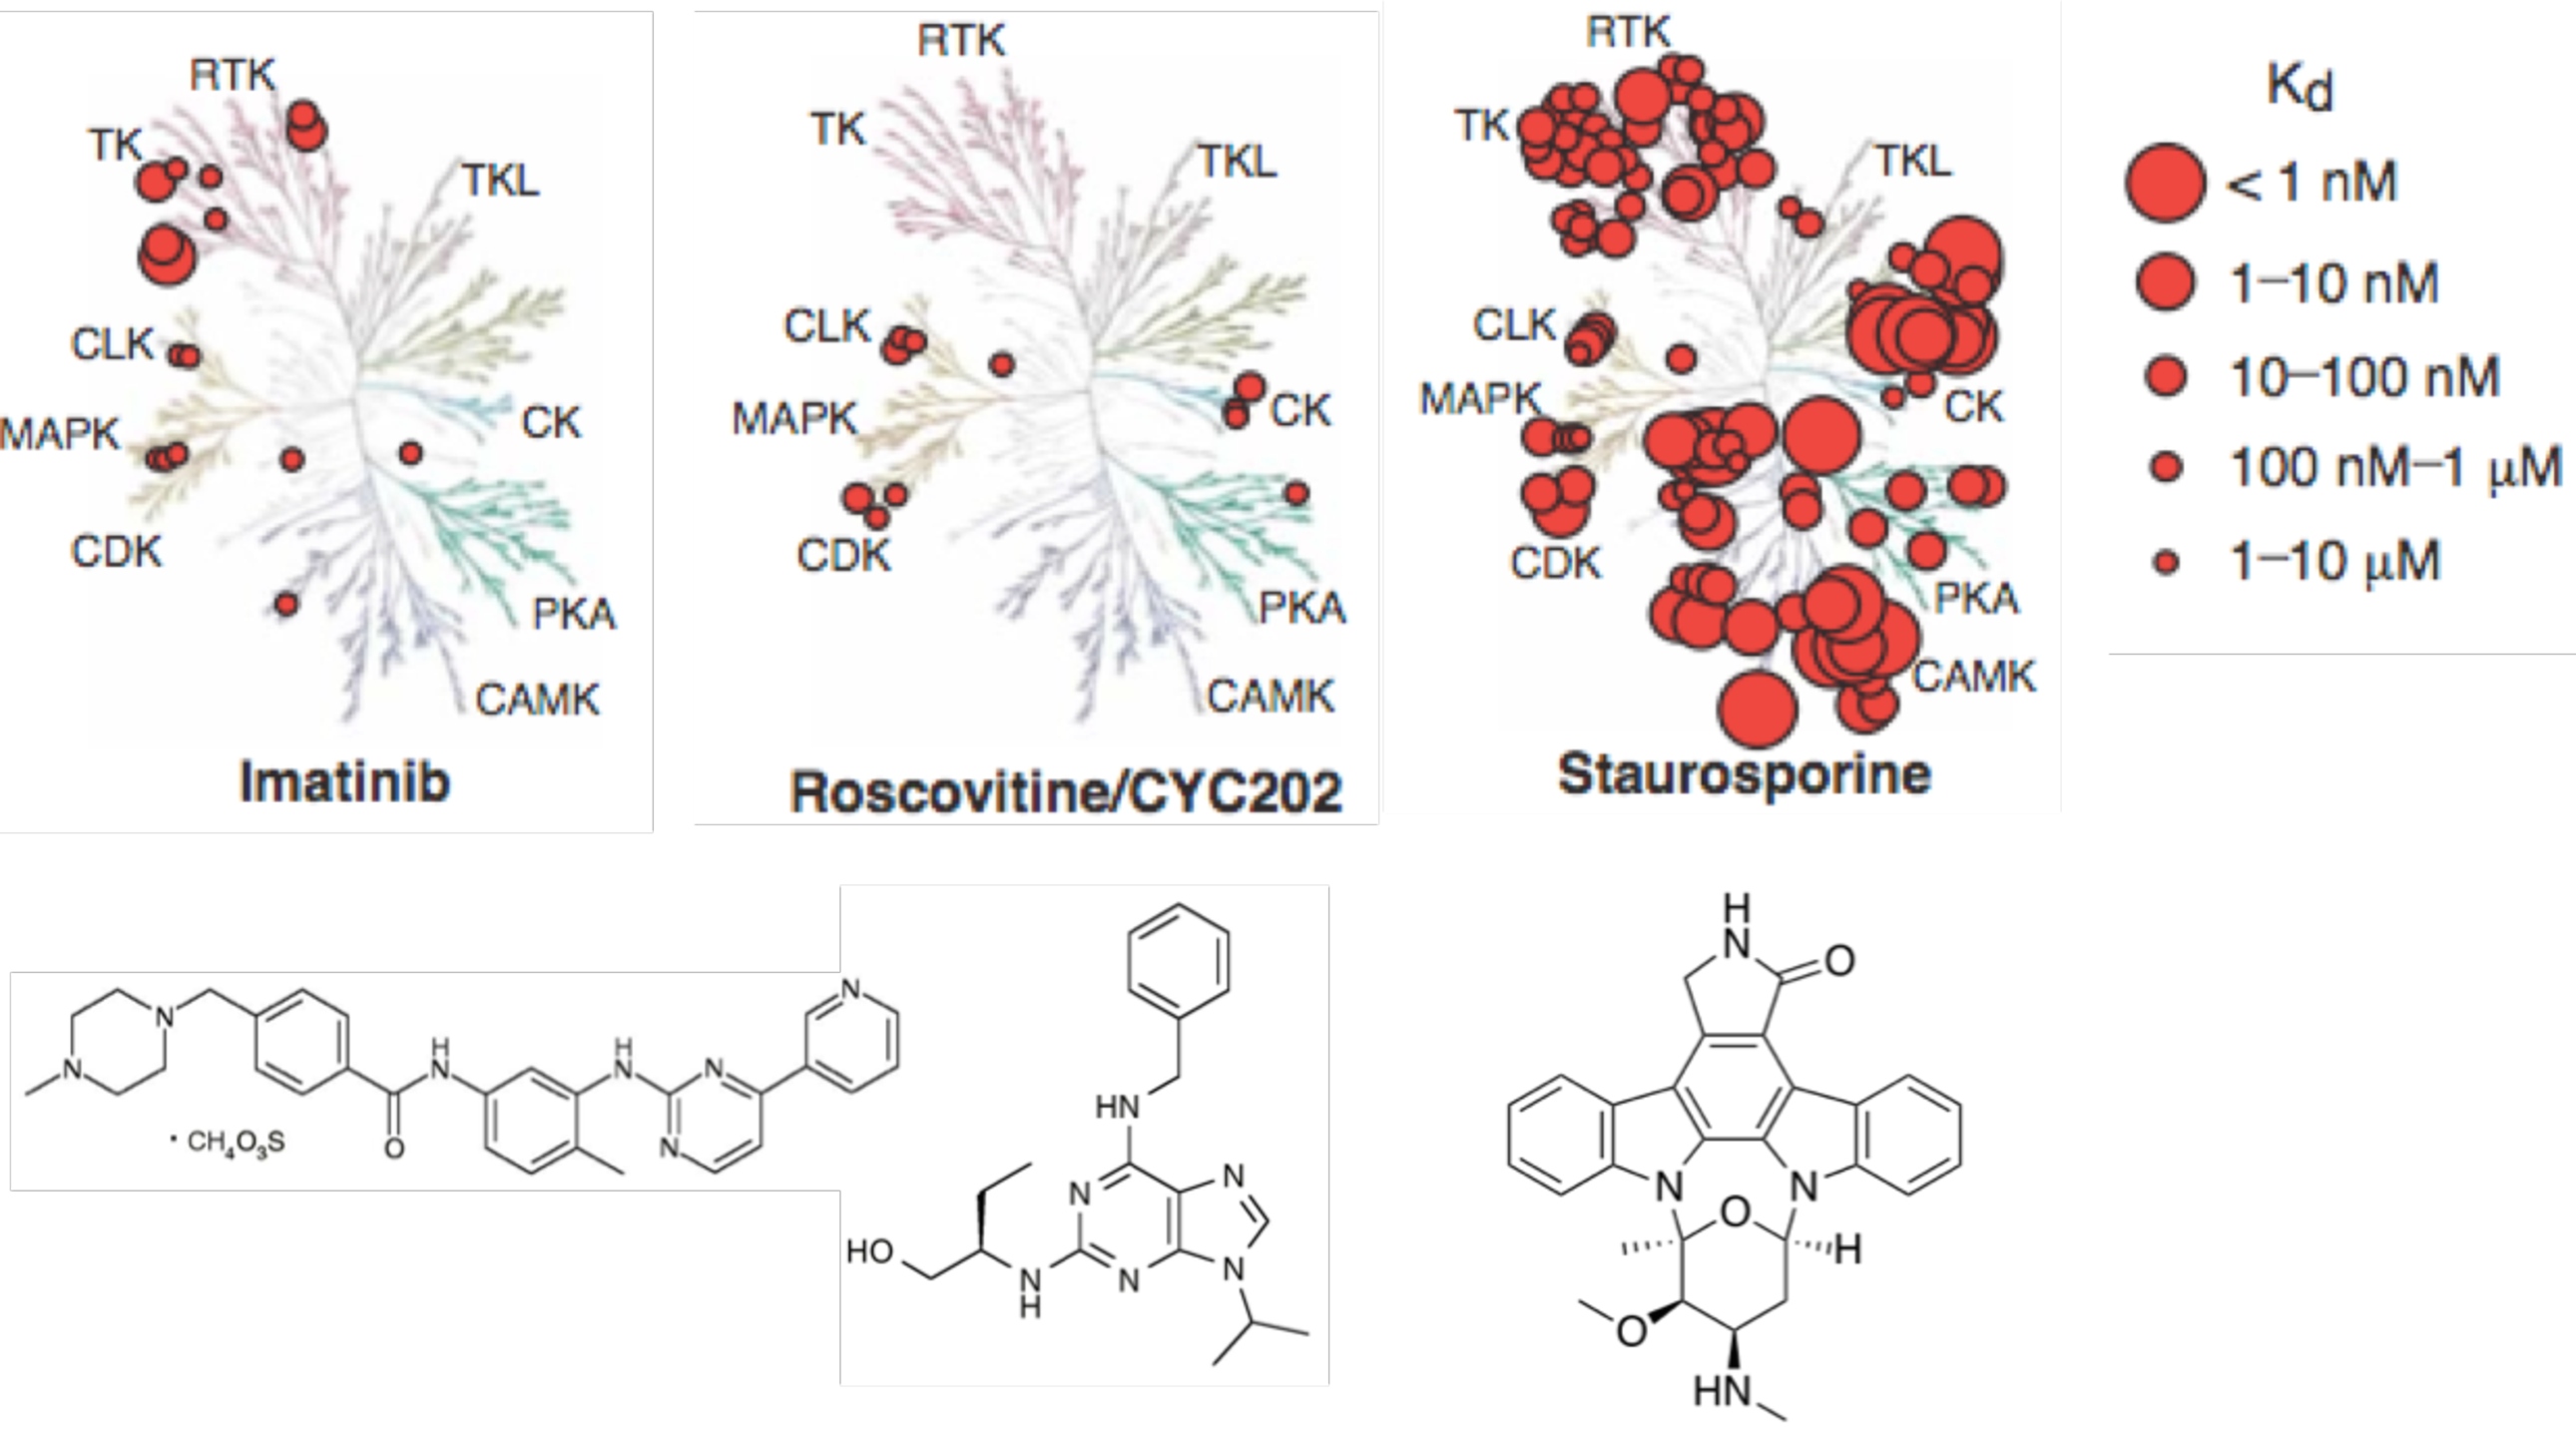
\includegraphics[width=0.44\textwidth]{figures/kinase-inhibitor-selectivity.pdf}
\vspace{-0.3cm}
\caption{\footnotesize \label{figure:kinase-inhibitor-selectivity} {\bf Kinase inhibitor selectivities are highly variable.}
Even targeted inhibitors like imatinib (\emph{left}) can inhibit a multitude of kinases; unselective inhibitors like staurosporine (\emph{right}) are highly toxic.
Adapted from~\cite{fabian:nature-biotech:2005:kinase-selectivity-map}.}
\end{wrapfigure}

We use massively parallel molecular dynamics simulations on the Folding@home worldwide distributed computing platform~\cite{shirts-pande:science:2000:folding-at-home}---the planet's largest computer for biology---to computationally map the conformations accessible to kinases and their associated energetics.
We have developed a tool (\emph{Ensembler}~\cite{ensembler}) to automate the modeling of human kinase catalytic domains onto all available kinase structures to broadly capture the variety of active and inactive conformations available to kinases, which are well-known to be highly conformationally heterogeneous. 
We then employ the Markov state modeling (MSM) approach I originally developed to study protein folding~\cite{chodera:2006:mms:long-time-dynamics,chodera:jcp:2007,noe:jcp:2011:msm-review} to extract distinct conformational states, energetics, and activation kinetics.
We are currently studying a number of kinases of interest to cancer and other diseases---ABL, SRC, MEK, MTOR, AURKA, DDR1, CK2, and SYK---and plan to extend this approach to all human kinases over the next two years.

To exploit these conformational and energetic maps of kinase conformations to understand kinase inhibitor affinity and selectivity, as well as facilitate the engineering of new selective inhibitors, we have developed a new generation of quantitatively accurate physical models based on alchemical free energy calculations~\cite{chodera:curr-opin-struct-biol:2011:drug-discovery}.
These methods use molecular mechanics forcefields to rigorously compute binding affinities that include all relevant statistical mechanical effects, including entropic and enthalpic contributions.
To make these techniques fast enough for practical use, we have built a new open-source GPU-accelerated code {\sc YANK}~\cite{wang:jcamd:2013:yank}.
{\sc YANK} combines numerous algorithmic improvements we have previously developed to achieve quantitative accuracy~\cite{mobley-chodera-dill:2006:jcp:orientation-restraints,mobley-chodera-dill:2007:jctc:confine-and-release,shirts-mobley-chodera-pande:2007:jpcb:dispersion-corrections,chodera:jcp:2007,shirts-chodera:jcp:2008:mbar,noe:jcp:2011:msm-review,ncmc,chodera-shirts:jcp:2011:gibbs} into a single code, and has an open architecture that allows critically-needed new algorithms to deal with kinase-specific effects to be easily developed, implemented, and validated.

In addition to allowing for accurate inclusion of the reorganization energy for different kinases, our kinase MSMs also reveal opportunities for allosterically targeting kinases by identifying conformations that expose otherwise cryptic binding sites that are not visible in crystallographic structures unless an allosteric inhibitor has already been identified and cocrystallized~\cite{bowman-geissler:pnas:2012:cryptic-allosteric-sites}.
As few allosteric kinase inhibitors have been identified to date, this represents an emerging opportunity for engineering new classes of effective therapeutics for cancer.

%%%%%%%%%%%%%%%%%%%%%%%%%%%%%%%%%%%%%%%%%%%%%%%%%%%%%%%%%%%%%%%%%%%%%%%%%%%%%%%%
% FIGURE: KINASE CONFORMATIONAL SELECTION
\begin{figure}[tb]
\begin{centering}
\begin{overpic}[scale=0.22]{figures/src-abl-comparison-2}\put(-10,0){\bf A}\end{overpic}
\begin{overpic}[scale=0.17]{figures/lee-craik-selectivity-image.pdf}\put(0,0){\bf B}\end{overpic}
\begin{overpic}[scale=0.29]{figures/overall-binding-free-energy.pdf}\put(0,0){\bf C}\end{overpic}

\end{centering}
\vspace{-0.1cm}
\caption{\footnotesize {\bf Conformational selection of kinase inactive states as a mechanism for inhibitor selectivity.}
{\bf (A)} Crystal structures of imatinib bound to Abl and Src show almost no differences in binding contacts or structure, despite the large 4.7 kcal/mol difference in selectivity.
{\bf (B)} Cartoon depiction of multiple conformational states with differing inhibitor binding competence (from Ref.~\cite{craik:2009:science:trapping-moving-targets}).
The arrow (E) denotes the reorganization free energy required to adopt a particular conformational state. For inhibitor (blue) to bind the the binding-competent conformation (red), an energetic penalty must be paid to confine the kinase to the binding-competent state; favorable binding free energy can then cause this conformation to become the new lowest free energy ``ground state''.
{\bf (C)} Illustration of how reorganization energy (red) and binding free energy (blue) give opposing contributions to overall binding free energy (black).
\label{figure:kinase-conformational-selection}}
\vspace{-0.4cm}
\end{figure}
%%%%%%%%%%%%%%%%%%%%%%%%%%%%%%%%%%%%%%%%%%%%%%%%%%%%%%%%%%%%%%%%%%%%%%%%%%%%%%%%

\emph{Predicting the emergence of mutational resistance.}
While drug resistance can emerge via multiple mechanisms, mutations in the therapeutic target drive the emergence of drug resistance in many patients; in commonly-targeted kinases such as Abl, missense mutations are responsible for resistance in as much as 90\% of cases~\cite{sawyers:cancer-cell:2002:abl-resistance}.
Developing a quantitative and predictive understanding for how these inhibitors elicit resistance through mutational mechanisms would be of immense value, allowing the rapid design of second-generation inhibitors to circumvent resistance, the exploration of therapeutic combinations to minimize the emergence of resistance, and potentially the development of new therapeutics unlikely to elicit resistance.

To predict resistance using physical modeling techniques, {\bf we hypothesize that resistance mutations ablate inhibitor binding affinity while maintaining some physically computable surrogate for activity}, such as ATP and substrate peptide binding affinities.
This allows us to compute a \emph{resistance index} for each possible point mutation, and to construct enhanced sampling schemes that selectively search for point mutations that maximize the resistance index.
We are currently building a framework to perform these calculations using our GPU-accelerated alchemical binding free energy code YANK~\cite{yank}, using Abl and Aurora kinases as model systems.
Predicted resistance mutations will be compared with clinically-identified lists of mutations, as well as tested in the laboratory through engineering these mutations into kinase catalytic domains that can be expressed recombinantly in bacteria.
We have developed an automated fluorescence assay to perform affinity measurements against a variety of small molecule kinase inhibitors of clinical interest, and use activity assays to determine whether our hypothesis regarding physical surrogates for activity is valid for individual kinases.

\emph{Predicting drug sensitivity and resistance in patient tumors.}
The ever-decreasing cost of next-generation sequencing technologies has spurred the deep sequencing of patient tumors with the goal of improving patient therapeutic outcomes by individually tailoring treatment plans to the specific genetic alterations found in that patient's cancer---potentially even only in small subpopulations of tumor cells.
While this development will undoubtedly revolutionize cancer therapy, there is a great deal of work left to be done over the next decade to connect tumor alterations to optimal therapeutic plans.

In particular, the problem of whether missense mutations in therapeutic targets represent resistance, neutral, or sensitizing mutations is of tremendous interest, as this knowledge could significantly shape therapeutic approaches.
Though many common mutations have been observed (and, less frequently, characterized biochemically and in cell lines)---such as the T315I gatekeeper mutation in Abl, which causes resistance to first-generation targeted inhibitors---the long tail of infrequently observed mutations essentially ensures that it will be impossible to catalog mutations presented in more than a minor fraction of cancers.

We take a two-pronged approach to predicting the therapeutic resistance or sensitivity of patient-derived tumor mutations:
First, we utilize the computational model built to predict the emergence of mutational resistance to identify potential resistance mutations (mutations that ablate inhibitor affinity while maintaining some surrogate for activity), and test these by engineering these mutations into bacterially-expressing kinases in our laboratory.
Success of this computational model in identifying mutations that cause resistance or susceptibility could eventually aid the development of individually-tailored treatment plans that maximize therapeutic success, avoiding drugs for which intrinsic resistance (even at the subclonal level) already exists, or employing combinations of therapeutics capable of overcoming inherent resistance.

Second, we are developing an automated high-speed cell-free expression pipeline that would allow mutant kinases to be engineered, expressed, and assayed against all available clinical kinase inhibitors within a day.
New cost-effective cell-free expression technologies based on S12 extracts and fed by glucose~\cite{kim_simple_2006,calhoun_economical_2008} allow for inexpensive and rapid scalable production of many proteins.
Aided by an FGI Rapid Response grant, our laboratory is currently exploring the automated optimization of these techniques (with GFP fluorescence or mass spectrometry as a readout) using machine-learning algorithms based on Gaussian processes to improve yields for kinase domains represented in the IMPACT assay to allow the production of kinases containing engineered patient mutations in a matter of hours.
Kinase production would be immediately followed by the fluorescence assay of kinase inhibitor affinity against all FDA-approved kinase inhibitors to aid the determination of whether inhibitors clinicians would like to use would be effective in light of tumor-specific mutations.
We anticipate this would allow us to reduce the entire engineering and assay pipeline to turn around sensitivity/resistance results within a single day, which is sufficiently short to have substantial impact on therapeutic decisionmaking.

\vspace{-0.3cm}
\subsubsection*{Rational design of anticancer therapeutics}
\vspace{-0.3cm}


\vspace{-0.3cm}
\subsubsection*{New biophysical measurement technologies}
\vspace{-0.3cm}

Due to its importance in drug design and the parameterization and validation of computational models for drug discovery, our lab is heavily invested in the development and extension of new biophysical measurement techniques capable of providing useful information about biomolecular energetics and ligand interactions.

{\bf Arrayed nanocalorimetry.}
%This includes everything from the development of new measurement technologies (such as an {\bf arrayed nanocalorimeter} under development with partners from Keysight Technologies) to the development of 

%\subsubsection*{Single-molecule experiments}

\subsection*{Major collaborative projects}

\subsubsection*{Selective inhibition of protein methyltransferases (Minkui Luo, MSKCC)}
\vspace{-0.3cm}
Protein lysine methyltransferases (PKMTs) regulate numerous epigenetic processes, and there is increasing evidence for their dysregulation playing a role in cancer through downregulation of tumor suppressors or upregulation of oncogenes that promote cancer progression and proliferation~\cite{Copeland:2009:Nat.Rev.DrugDiscov.}.
There is tremendous interest in utilizing a variety of selective inhibitors to illuminate the role of PKMTs in disease and develop potential therapeutics, but few such inhibitors exist.
Like kinases, PKMTs are conformationally heterogeneous, providing an opportunity to exploit binding to distinct conformations to achieve selectivity.
Funded by a STARR Cancer Consortium grant with Minkui Luo, we are working to apply the same methodology used for designing selective kinase inhibitors to aid the Luo lab in developing useful chemical probes for elcudiating PKMT function.

\vspace{-0.5cm}
\subsubsection*{GPCR dynamics and activation (Scott Blanchard and Harel Weinstein, WCMC)}
\vspace{-0.3cm}
G-protein coupled receptors (GPCRs) represent a significant fraction of all drug targets, and are gradually being recognized as playing important roles in tumor progression and metastasis~\cite{Dorsam:2007:Nat.Rev.Cancera}.
In collaboration with Scott Blanchard and Harel Weinsteil (WCMC), we are working to illuminate the detailed conformational changes involved in biased agonism and signal transduction using massively parallel simulations on Folding@home that will bridge from static crystal structures to dynamic single-molecule FRET data collected in the Blanchard lab.
The resulting detailed model will aid the subsequent design of new GPCR biased agonists and inhibitors.

\vspace{-0.5cm}
\subsubsection*{Activating mutants of MTOR (James Hsieh, MSKCC)}
\vspace{-0.3cm}
The MSK-IMPACT panel has identified a large diversity of tumor-associated mutations in the MTOR gene, an atypical serine/threonine kinase that acts as a master growth regulator.
By engineering these mutations into cell lines, the Hsieh lab has demonstrated that many of these mutations are activating, and identified several distinct mechanistic classes of mutations.
Funded by an FGI grant, we are working with the Hsieh lab to elucidate the structural and energetic ramifications of these mutations with the goal of identifying opportunities for therapeutic intervention.

\vspace{-0.5cm}
\subsubsection*{Allosteric and slow off-rate inhibition of CK2 and SYK (Melissa Vasbinder, AstraZenea)}
\vspace{-0.3cm}
In a closed system, the binding affinity of an inhibitor for its target fully determines target inhibition, but in an open system such as a cell where drugs can be exported or metabolized and cleared from the blood, the off-rate of an inhibitor can more directly determine the efficacy of inhibition~\cite{copeland:nrdd:2007:residence-time}.
Through a funded collaboration with Astra-Zeneca, we are exploring the mechanistic origins of surprisingly slow off-rate inhibitors they discovered for CK2 (now a dead project), and examining opportunities for engineering allosteric inhibitors or slow-off-rate inhibitors for SYK.

\vspace{-0.3cm}
\subsubsection*{Protonation state effects in kinase inhibitor recognition (Marilyn Gunner, CCNY)}
\vspace{-0.3cm}
Recently, the complicated role that protonation states play in the binding of imatinib to Abl has suggested that both \emph{equilibrium mixtures} of protonation states and \emph{changes} in protonation state upon binding are relevant to accurately describing inhibitor binding~\cite{szakacks:j-med-chem:2005:acid-base-profiling-of-imatinib,seeliger:2007:structure:imatinib-binding,roux:pnas:2013:gleevec-selectivity}, posing an enormous challenge to computational drug design paradigms, which do not consider protonation state effects explicitly.
We believe protonation states may play a much larger role in both on- and off-target kinase inhibition than previously appreciated, since over \emph{half} of all FDA-approved small molecule kinase inhibitors have two or more protonation states predicted to be accessible during binding.
Working with Marilyn Gunner (CCNY), who has extensive experience in protonation state modeling in proteins, we are embarking on a large-scale effort to elucidate the role of protonation state effects in kinase inhibitor binding and explicitly allow protonation state effects to be considered in inhibitor design and profiling of off-target effects.
We plan to apply for NIH funding for this project in early 2016.

\vspace{-0.3cm}
\subsubsection*{MHC-peptide-TCR interactions (David Scheinberg, MSKCC)}
\vspace{-0.3cm}

Recently, the development of immuotherapies that promote the recognition of mutated tumor antigen has spurred the desire to develop quantitative, predictive models for for the association of major histocompatibility complex (MHC) with T cell receptors (TCR) mediated by antigen peptide binding interactions, in order to permit the development of novel biologics that may be useful in cancer treatment.
These biologics may be recombinant variants of TCRs, TCR-mimicking antibodies (TCRm), or even synthesized antigen peptides for use as potential vaccines.
In all of these cases, a detailed, accurate model for the affinity of the MHC-peptide-TCR/TCRm complex (including the details of an individual's MHC variants) for both cancer and self antigen peptides is essential.

\begin{wrapfigure}[15]{right}{0.40\textwidth}
\vspace{-2.6cm}
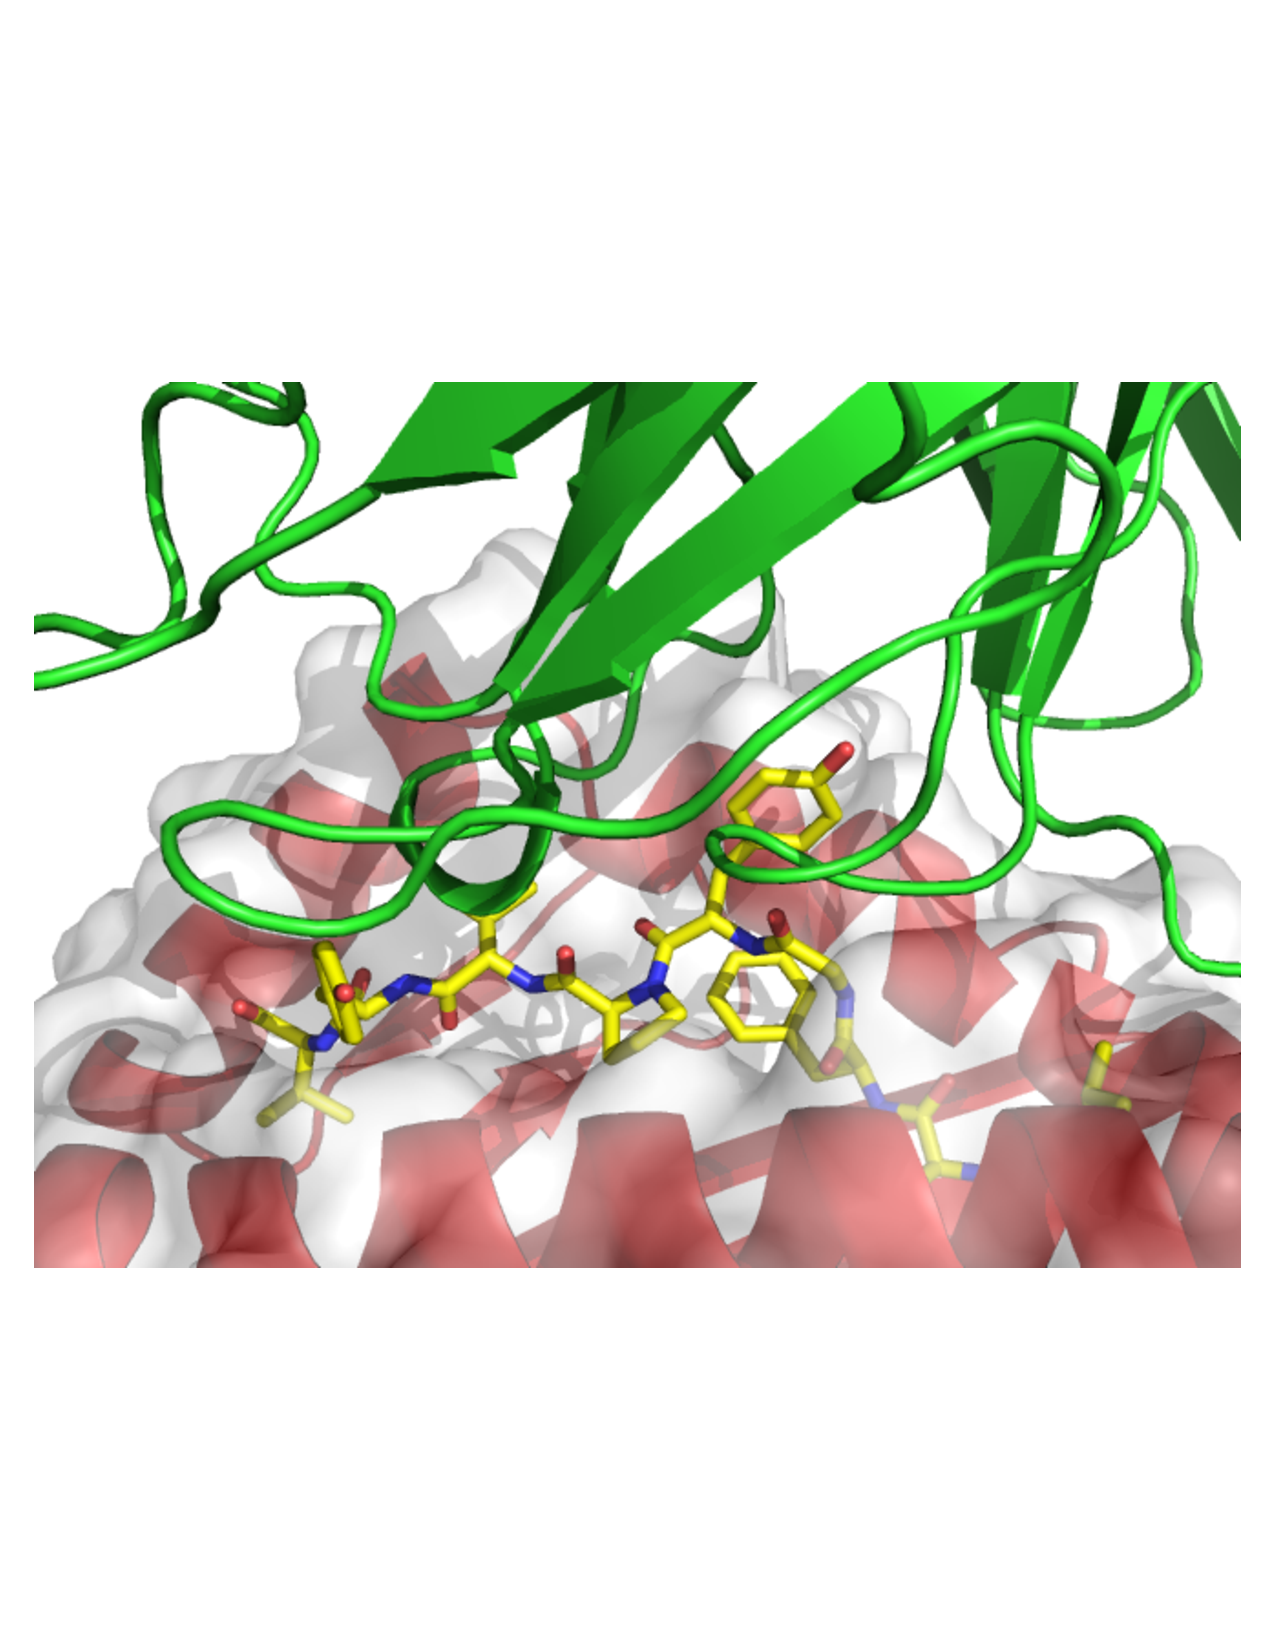
\includegraphics[width=0.38\textwidth]{figures/1AO7.pdf}
\vspace{-2.5cm}
\caption{\footnotesize \label{figure:mhc-peptide-tcr} {\bf MHC-peptide-TCR complex.}
Human major histocompatibility complex (MHC; \emph{red}) HLA-A2 and T cell receptor (TCR; \emph{green}) is shown in complex with the viral TAX peptide (LLFGYPVYV; \emph{yellow}) [rcsbid:1AO7].}
\end{wrapfigure}

While simple experiment-derived additive models derived from experimental data have been proposed~\cite{Birnbaum:2014:Cell}, these models are insufficiently accurate for the purpose of therapeutic engineering.
We are working with Ron Gejman and David Scheinberg at MSKCC to utilize atomistically detailed free energy calculations for this purpose.
First, we are exploring what biophysical detail is necessary to recapitulate known affinities for the MHC-peptide-TCR ternary complex.
Next, we will utilize advanced techniques for sampling over sequence space to perform the computational equivalent of evolution selection experiments, selecting for peptide sequences that bind tightly to specific MHC-TCR complexes.
In addition to aiding the development of novel therapeutics, accurate computational models of MHC-peptide-TCR complex affinity will also be useful in predicting the degree of therapeutic response from individual tumor sequences.

\vspace{-0.3cm}
\subsubsection*{Human serum albumin binding and interference (Ron Blasberg, MSKCC)}
\vspace{-0.3cm}

\begin{wrapfigure}[13]{right}{0.40\textwidth}
\vspace{-2.3cm}
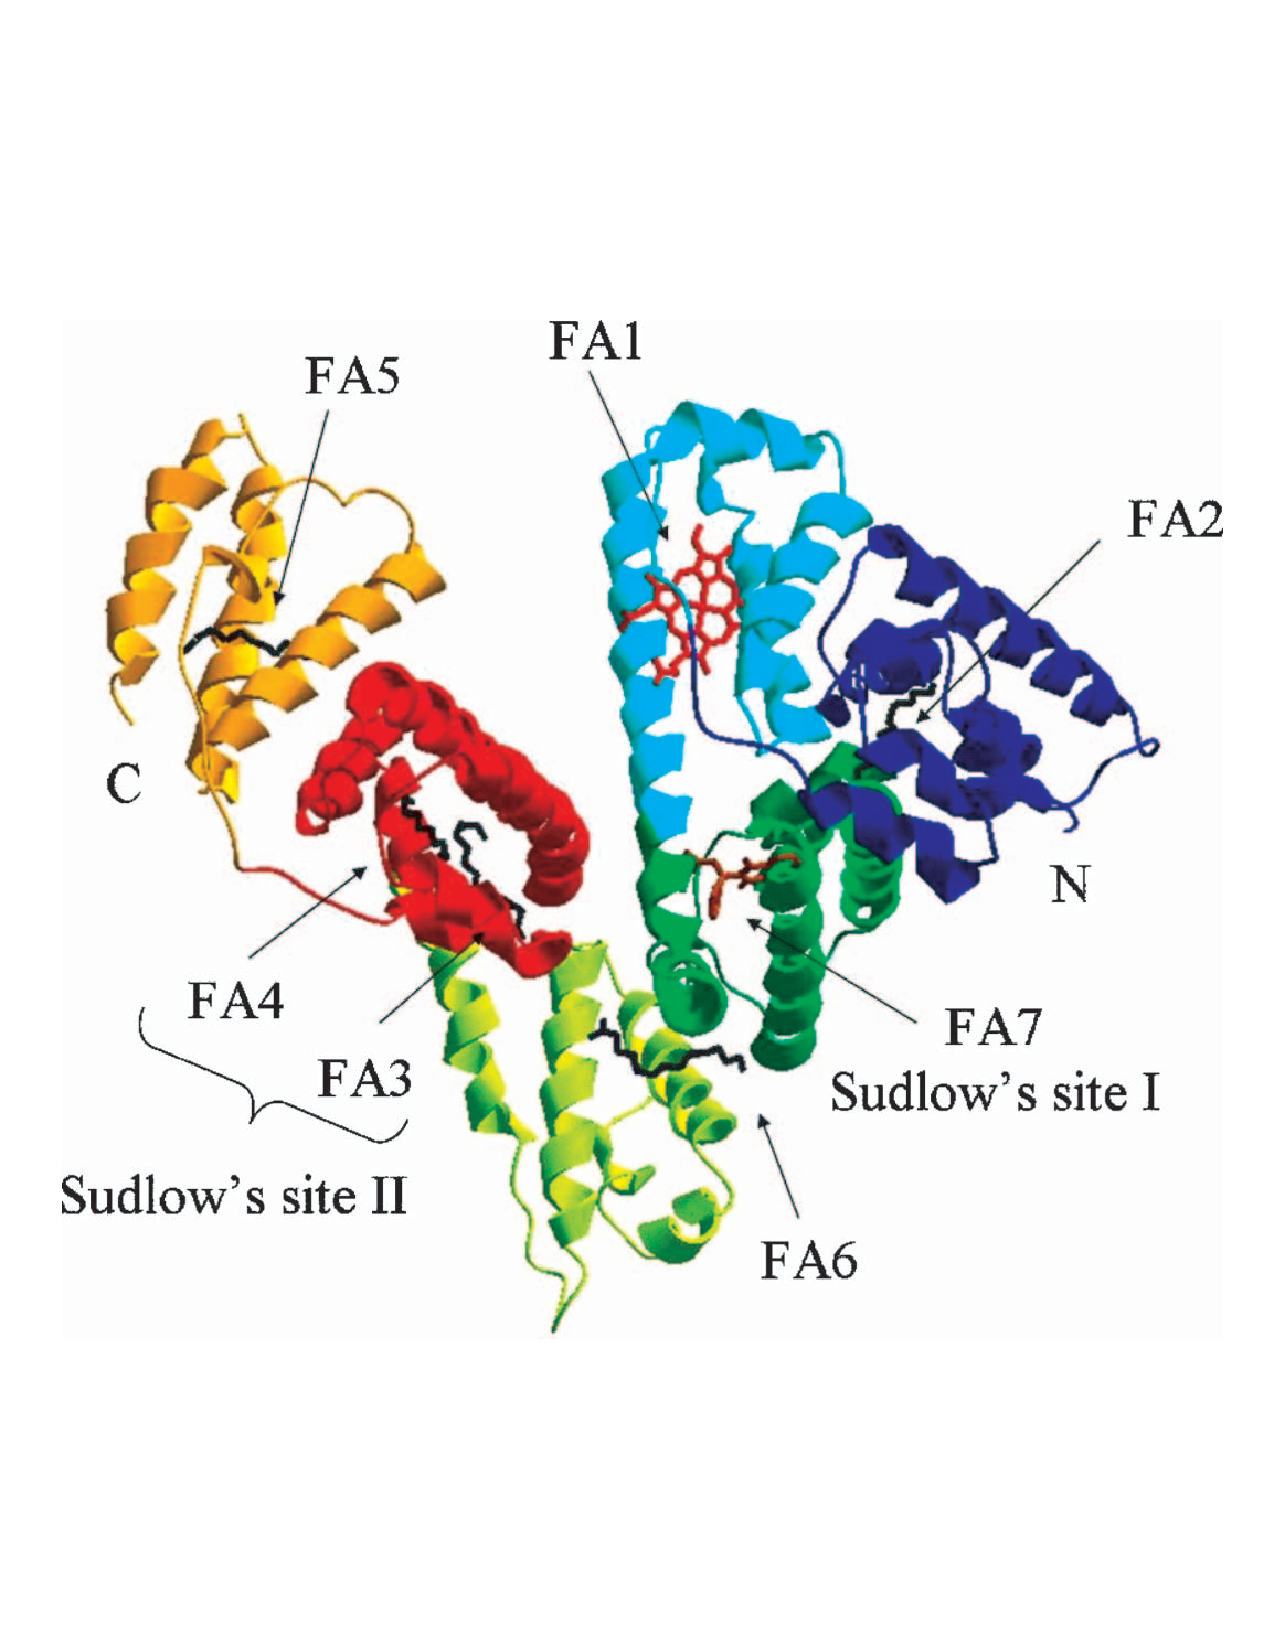
\includegraphics[width=0.38\textwidth]{figures/hsa-binding-sites.pdf}
\vspace{-2.5cm}
\caption{\footnotesize \label{figure:hsa} {\bf Human serum albumin.}
Characterized drug and fatty acid binding sites are shown.
Adapted from~\cite{fasano:iubmb-life:2005:hsa-review}.}
\end{wrapfigure}

Binding to the abundant human serum protein albumin (HSA, Figure~\ref{figure:hsa}) is well-known to modulate the pharmacokinetics of drugs, including common drugs such as aspirin and ibuprofen~\cite{fasano:iubmb-life:2005:hsa-review}.
While this may sometimes be advantageous, in many cases, HSA binding prevents accumulation of bioactive conformations at target sites of interest.
The Blasberg lab encountered just such a case with a radiolabeled dye molecule intended for the visualization of CXCR-expressing cells in brain cancer associated with poor prognosis: While the molecule binds CXCR effectively and crosses the blood-brain barrier, the molecule binds HSA to a degree that useful quantities cannot accumulate in the brain.

To enable these radioligands to be useful in imaging, we are working with the Blasberg lab to identify safe, well-tolerated drugs that could be coadministered with the label compound to saturate the HSA binding site and ensure sufficient compound can reach target receptors in the brain.
While complicated by the fact that HSA has at least seven characterized binding sites (Figure~\ref{figure:hsa}), this could function as a novel approach to modulating the pharmacokinetics of HSA-binding drugs or imaging agents.
Our approach first aims to identify the binding sites to which the radioimaging compound has high affinity using a novel GPU-accelerated binding free energy computation technique we developed for characterizing multiple weak binding events.
We then utilize automated isothermal titration calorimetry and fluorescence competition assays to experimentally verify both binding sites (using well-characterized reporter compounds) and compound affinity.
Once candidate well-tolerated competitive drugs are identified, Blasberg lab will carry out subsequent experiments in rodents to demonstrate the practicality of this approach.

We are currently developing this concept into a funding proposal with James Fraser (UCSF), who will use room-temperature X-ray crystallography to provide complementary experimental validation of our findings.

%%%%%%%%%%%%%%%%%%%%%%%%%%%%%%%%%%%%%%%%%%%%%%%%%%%%%%%%%%%%%%%%%%%%%%%%%%%%%%%%%%%%%%%%%%%%%%%%%%%%%%
% BIBLIOGRAPHY
%%%%%%%%%%%%%%%%%%%%%%%%%%%%%%%%%%%%%%%%%%%%%%%%%%%%%%%%%%%%%%%%%%%%%%%%%%%%%%%%%%%%%%%%%%%%%%%%%%%%%%

\eject
\footnotesize
\setlength{\parskip}{0em}
\renewcommand{\baselinestretch}{1.0}
\bibliographystyle{prsty} 
\bibliography{chodera-research.bib}

\end{document}
